\documentclass[nobib]{tufte-book-tai}

% -------------------------------FONTS--------------------------------- %
%% latex font  
% \usepackage[T1]{fontenc} %computer roman font
% \usepackage[utf8]{inputenc} %computer roman font
% \usepackage{lmodern} %computer roman font

%% Tufte's ETBembo Font! Build with xelatex
% \usepackage{fontspec} %tufte font
% \setmainfont{ETBembo}%[Mapping=TeX-text] %tufte font
%% this fixes a bug with Bembo: (https://github.com/Tufte-LaTeX/tufte-latex/issues/64)
% \renewcommand\allcapsspacing[1]{{\addfontfeature{LetterSpace=15}#1}}
% \renewcommand\smallcapsspacing[1]{{\addfontfeature{LetterSpace=10}#1}}

% -------------------------------PREAMBLE--------------------------------- %
\usepackage{amsmath}
\usepackage{amssymb}
\usepackage{cancel}
\usepackage{amsthm}
\usepackage{mathrsfs}
\usepackage[dvipsnames]{xcolor}
\usepackage{graphicx}
\usepackage{epigraph}
\usepackage{booktabs}
\usepackage{relsize}
\usepackage{hyperref}
\usepackage{multicol}
  \setlength{\columnsep}{3cm}
\usepackage{floatrow}
	\newfloatcommand{capbtabbox}{table}[][\FBwidth]
\usepackage{kbordermatrix}
\usepackage{transparent}
\usepackage[normalem]{ulem}
\hypersetup{colorlinks} 
\hypersetup{ %uncomment to override tufte colors
    colorlinks=true,    
    %urlcolor=ProcessBlue,
    linkcolor =RubineRed,
    citecolor=RubineRed
}

\usepackage{array}

\usepackage[shortlabels]{enumitem}
\setlist[enumerate]{leftmargin=*, align=left}
\setlist[itemize]{topsep=1ex}

% Diagram Packages: Need to keep in this order.
\usepackage{tikz}
\usetikzlibrary{cd,calc, arrows, shapes, matrix, positioning, intersections, decorations.markings, arrows.meta, decorations.pathmorphing}
  \tikzcdset{arrow style=tikz, diagrams={>=stealth}}
	\tikzstyle{vertex}=[fill=black,circle,scale=0.6]
	\tikzset{thick/.style={line width=.6mm}}
  \tikzstyle{tensor}=[circle,thick,draw=black,fill=blue!60!green!40!white,minimum size=4mm]
  \tikzstyle{witharrow} = [thick,decoration={
      markings,mark=at position 0.75 with {\arrow[scale=1.5,>=stealth]{>}}},postaction={decorate}]
  \tikzstyle{littletensor}=[circle,thick,draw=black,fill=red!30,minimum size=.5mm] 

% ----------------------------------Commands---------------------------------- %

% functional version of the old command $\iso$. This takes an argument for what goes over the arrow.
\newcommand{\ar}[1]{\xrightarrow{\ensuremath{#1}}}


% Shorthand
\newcommand{\V}{\mathcal{V}}
\renewcommand{\C}{\mathsf{C}}
\newcommand{\D}{\mathsf{D}}
\newcommand{\E}{\mathsf{E}}
\renewcommand{\o}{{\color{YellowOrange}o}}
\newcommand{\g}{{\color{Green}g}}
\newcommand{\p}{{\color{Purple}p}}
\newcommand{\<}{\langle}
\renewcommand{\>}{\rangle}
\newenvironment{bsmallmatrix}
  {\left[\begin{smallmatrix}}
  {\end{smallmatrix}\right]}
\let\emph\relax % there's no \RedeclareTextFontCommand
\DeclareTextFontCommand{\emph}{\bfseries}




% Categories and Operators
\newcommand{\End}{\operatorname{End}}
\newcommand{\op}{\operatorname{op}}
\newcommand{\tr}{\operatorname{tr}}
\DeclareMathOperator{\id}{id}
\DeclareMathOperator{\eval}{eval}

\newcommand{\adj}[4]{
\begin{tikzcd}[ampersand replacement=\&, column sep=4ex, cramped]
   #1 \colon #2	\ar[yshift=+.6ex]{r}
\& #3 \colon #4	\ar[yshift=-.4ex]{l}
\end{tikzcd}
}

% -----------------------------------Style------------------------------------ %
% --                                                                        -- %

\theoremstyle{plain}
\newtheorem{theorem}{Theorem}%[chapter]
\newtheorem{lemma}{Lemma}[chapter]
\newtheorem{proposition}{Proposition}[chapter]
\newtheorem{corollary}{Corollary}[chapter]
\newtheorem{takeaway}{Takeaway}%[section]


\theoremstyle{definition}
\newtheorem{definition}{Definition}[chapter]
\newtheorem{example}{Example}[chapter]
\newtheorem{remark}{Remark}[chapter]
\newtheorem{aside}{Aside}%[chapter]

% Named Theorems
\newtheorem{Yoneda}{Yoneda Lemma}[theorem]
\newtheorem{tych}{Tychonoff's Theorem}{\bfseries}{\itshape}
\newtheorem*{UP_vect}{Universal Property for Vector Spaces}{\bfseries}{\itshape}
\newtheorem*{UP_meet}{Universal Property for Free Meet Semilattices}{\bfseries}{\itshape}
\newtheorem*{UP_join}{Universal Property for Free Join Semilattices}{\bfseries}{\itshape}
\newtheorem*{UP_cocomplete}{Universal Property for the Free Cocompletion of a Category}{\bfseries}{\itshape}
\newtheorem*{UP_complete}{Universal Property for the Free Completion of a Category}{\bfseries}{\itshape}
\newtheorem*{mainprocedure}{Main Procedure}{\bfseries}{\itshape}

% -----------------------------------Colors----------------------------------- %

\newcommand{\tai}[1]{{\color{cyan}#1}}
\newcommand{\green}[1]{{\color{Green}#1}}

% -------------------------------TUFTE INDEX--------------------------------- %


  
\title{The Lonnrot Language}
\author{Andrés Ricardo Garza Vela}


% -------------------------------EPIGRAPHS--------------------------------- %

%% latex style
\usepackage{epigraph}
\renewcommand{\epigraphflush}{flushleft}
\renewcommand{\sourceflush}{flushleft}

% Prints an epigraph and speaker in sans serif, all-caps type.
\newcommand{\openepigraph}[2]{
  {\Large
  \noindent{#1}\\% epigraph
  - {\itshape\noindent{#2}}% author
  } }

% ---------------------------------INDEX------------------------------------- %

\usepackage{makeidx}
\makeindex

% ----------------------------BEGIN DOCUMENT--------------------------------- %

\begin{document}
%\raggedbottom
\maketitlepage

% \let\cleardoublepage\clearpage %this gets rid of blank pages. comment out for actual printing


% ----------------------------COPYRIGHT PAGE--------------------------------- %
\newpage
\begin{fullwidth}
~\vfill
\thispagestyle{empty}
\setlength{\parindent}{0pt}
\setlength{\parskip}{\baselineskip}
Copyright \copyright\ \the\year %\ \thanklessauthor

\par \thanklessauthor

\par\smallcaps{All Rights Reserved}


%\par A dissertation submitted to the Graduate Faculty in Mathematics in partial fulfillment of the requirements for the degree of Doctor of Philosophy, The City University of New York

\par A report written for the course of Compiler Design at ITESM

\end{fullwidth}

\clearpage



% ----------------------------------TOC------------------------------------- %
\setcounter{page}{3}
\setcounter{tocdepth}{2}
\tableofcontents

\frontmatter
% ------------------------------FRONT MATTER--------------------------------- %
\setcounter{page}{5}

\chapter*{About the Lonnrot Language}
\addcontentsline{toc}{chapter}{About the Lonnrot Language}

% Discuss objective
% Discuss area

%\chapter*{Acknowledgments}
\addcontentsline{toc}{chapter}{Acknowledgments}

% Acknowledgment ideas:
% My family, obviously
% Eduardo for his insight, patience and friendship
%
% Impersonal:
% Anne Ogborn: for her guidance in logic programming and her
% reference to Clocksin and Mellish's ISO Prolog
%
% The Reasoned Schemers, for their continued work on miniKanren
%
% Edward Tufte, for his insight into data presentation
% Likewise to, Tai-Danae Bradley, for her beautiful tufte-latex inspired work
%
% José Manuel Calderón Trilla and the folks at UMD's CMSC430


% ---------------------------------CHAPTERS---------------------------------- %
\mainmatter
\setcounter{secnumdepth}{2}

%chapter 1
\chapter{Tetragrammaton}\label{ch:TFE}

\epigraph{The s-expression syntax dates back to 1960. This syntax is often controversial amongst programmers. Observe, however, something deeply valuable that it gives us. While parsing traditional languages can be very complex,
  parsing this syntax is virtually trivial.}{Shriram Krishnamurthi~\cite{krishnamurthi20}}

%This chapter outlines the main components of the language in the form of \textit{tokens}, \textit{syntax diagrams} and \textit{semantics}. Then, it presents some core functions, which will serve as a foundation for a sort of
%standard library in later chapters. This discussion is finally rounded out with the consideration of \textit{data types} and \textit{data structures} that are a part of the language.


% Mention we won't deal with strings for now
% Mention anyChar is literally any char, digit is 0 to 9

\section{Basic Elements}\label{sec:ch1_BE}
\setlength{\grammarparsep}{8pt} % increase separation between rules
\setlength{\grammarindent}{8em} % increase separation between LHS/RHS
\begin{grammar}
    <datum> ::= <boolean>
    \indalt <character>
    \indalt <variable>
    \indalt <string>
    \indalt <number>
    \indalt <list>

    <variable> ::= <initial> <subsequent>*

    <initial> ::= <letter> | `!' | `$' | `&' | `*' | `/' | `:' | `<' | `=' | `>' | `?' | `~' | `_' | `^'

    <letter> ::= a | \ldots | z | A | \ldots | Z

    <boolean> ::= \texttt{\#t} | \texttt{\#f}

    <number> ::= <integer> | <decimal>

    <integer> ::= <digit>+

    <decimal> ::= <integer> `.' <digit>+

    <char> ::= `\#' <any-character>

    <list> ::= (<datum>*)
    \indalt (<datum>+ . <datum>)
\end{grammar}


\section{Syntax}\label{sec:ch1_Syn}
\setlength{\grammarparsep}{8pt} % increase separation between rules
\setlength{\grammarindent}{8em} % increase separation between LHS/RHS
\begin{grammar}
    <program>     ::= <form>*

    <form>        ::= <definition> | <expression>

    <definition>  ::= (\texttt{define} <variable> <expression>)

    <expression>  ::= <constant>
    \indalt <variable>
    \indalt (\texttt{quote} <datum>)
    \indalt (\texttt{fresh} <formals> <expression> <expression>*)
    \indalt (\texttt{==} <expression> <expression>)
    \indalt (\texttt{run} <digit> <formals> <expression>)
    \indalt (\texttt{lambda} <formals> <expression> <expression>*)
    \indalt (\texttt{if} <expression> <expression> <expression>)
    \indalt (\texttt{set!} <variable> <expression>)
    \indalt <application>

    <constant>    ::= <boolean> | <number> | <char> | <string>

    <formals>     ::= <variable>
    \indalt (<variable>*)
    \indalt (<variable> <variable>* . <variable>)

    <application> ::= (<expression> <expression>*)
\end{grammar}

\clearpage

\section{Syntax Diagrams}\label{sec:ch1_SD}
\railalias{dol}{\$}
\railalias{amp}{\&}
\railalias{til}{\~{}}
\railalias{uscore}{\textunderscore}
\railalias{caret}{\^{}}
\railalias{bs}{\char''5C}
\railterm{dol, amp, til, uscore, caret, bs}
\begin{rail}
  datum : boolean
  | character
  | variable
  | string
  | number
  | list
  ;

  boolean : '\#t' | '\#f' ;

  char : anyCharacter ;

  number : integer | decimal ;

  integer : digit + ;

  decimal : integer '.' digit + ;

  variable : initial (subsequent*) ;

  initial : letter | '!' | dol | amp | '*' | '/' | ':' | '<' | '=' | '>' | '?' | til | uscore | caret ;

  letter : [a--z] | [A--Z] ;


  list : '(' (datum *) ')' | '(' (datum +) '.' datum ')'

\end{rail}

\railalias{dol}{\$}
\railalias{amp}{\&}
\railalias{til}{\~{}}
\railalias{uscore}{\textunderscore}
\railalias{caret}{\^{}}
\railalias{bs}{\char''5C}
\railterm{dol, amp, til, uscore, caret, bs}
\begin{rail}
  program : form* ;

  form : definition | expression ;

  definition : '(' 'define' variable expression ')' ;

  expression : constant
  | variable
  | '(' 'quote' datum ')'
  | '(' 'fresh' formals expression (expression*) ')'
  | '(' '==' expression expression ')'
  | '(' 'run' digit formals expression ')'
  | '(' 'lambda' formals expression (expression*) ')'
  | '(' 'if' expression expression expression ')'
  | '(' 'set!' variable expression ')'
  | application ;

  formals : variable
  | '(' (variable*) ')'
  | '(' variable (variable*) '.' variable ')' ;

  application : '(' expression (expression*) ')' ;

\end{rail}


\clearpage

%chapter 2
\chapter{Red Scharlach}\label{ch:two}

% Values
\section{Operational Semantics}\label{sec:ch2_opsem}

% I/O

\clearpage

%chapter 3
\chapter{Execution}\label{ch:exe}

\newthought{Once we have translated code} what is left is evaluating it. In this
chapter, we discuss the implications of evaluating Lonnrot code: type checking,
runtime operations and how what concessions have to be made to represent an environment
in a setting such as x86 or a register-based virtual machine.

% c.4
\section{Semantics}\label{sec:ch3_semantics}
\subsection{Type Tags}
To be able to perform type-checking we must have a mechanism to distinguish values
at runtime. To that end, we use \textbf{type tags}. Under that premise, values are either
\textbf{immediates} or \textbf{pointers}.\marginnote{Immediates are called that way because they
  represent data that is storable in a machine word.}
The following table outlines the hierarchy and the corresponding tags used

\begin{center}
  \begin{tabular}[h]{c | c}
    \toprule
    \multicolumn{2}{c}{Immediates (end in 000)}\\
    \textbf{Type} & \textbf{Tag}\\
    \midrule
    Integer & 0000 0000 \\
    Char    & 0000 1000 \\
    True    & 0001 1000 \\
    False   & 0011 1000 \\
    EOF     & 0101 1000 \\
    Void    & 0111 1000 \\
    Empty   & 1001 1000 \\
    \bottomrule
  \end{tabular}
\end{center}

\begin{center}
  \begin{tabular}[h]{c | c}
    \toprule
    \multicolumn{2}{c}{Pointers (do not end in 000)}\\
    \textbf{Type} & \textbf{Tag}\\
    \midrule
    Box         & 001 \\
    Pair (Cons) & 010 \\
    Strings     & 011 \\
    Functions   & 100 \\
    \bottomrule
  \end{tabular}
\end{center}
\vspace{1cm}

To type check, then, is to emit code that:
\begin{itemize}
  \item Moves a value to a scratch register (\texttt{r9})
  \item \texttt{and}s this with a type mask (e.g.\ the type mask for an int is \texttt{1111})
  \item Compares the result with the type tag
  \item Generates a \texttt{jne} code that jumps to the runtime exception handler.
\end{itemize}
\vspace{1cm}

Type tagging raises the issue of compiler correctness due to limitations in representation.
\marginnote{Actually, the mere fact of storing integers within a machine word without any
implementation of bignums also does this, but alas.}
In Lonnrot Scheme \textit{there are integer overflows and underflows}, and the behavior is
the same as that of, say, C. Likewise, it speaks to some of the characteristics of the x86
architecture. The most obvious example of this is pointer tagging: choosing to represent
pointers as values with the last three bits set to things other than zero is not arbitrary.
This is because x86 is \textit{byte-addressable}, meaning that it is not possible for us to
accidentally ``step on'' another address by fiddling with the last three bits. We have thus
the ability to represent 8 different types of data with pointers.

In any case, further information about which primitives accept which type of data is given
in the Quick Reference~\ref{ch:quickref}.

\subsection{Function Calling}
Another important part of discussing the language's semantics is the issue of \textit{how} functions
are evaluated. Generally, there are three main issues at hand: (1) do we evaluate \textit{all} function
arguments before jumping to the function's code? (2) Which argument do we evaluate first? Should we
do this left to right? (3) Do we check if the function exists before or after evaluating the arguments?

To cut straight to the chase, the answer to those questions is: Lonnrot Scheme evaluates all of the
arguments before the jump, and it does so before checking if the function exists.
\marginnote{This is called, quite appropriately, \textbf{eval-apply} semantics of function application}
Regarding question number two, there is no particularly defined way to do this in Scheme, generally. However
Lonnrot Scheme evaluates arguments \textbf{left to right}.

% d.2
\section{Runtime and Memory}
The runtime allows us to perform certain operations that would otherwise require lots of assembly code.
The prime example of this is printing results, where we piggy-back on \texttt{printf} and a couple of
helper functions that allow for special formatting depending on the type of data to be represented. This
is especially handy because of type tagging: we can delegate the bit shifting required to produce an
actual value to the runtime instead of emitting more code ourselves (even if it is possible to do so).

Equally important though is the fact that  the runtime allows us to allocate heap memory through the use of
\texttt{malloc}.
This should make it apparent why the discussion on representing memory during compilation was
so short: because we are already thinking in terms of the actual hardware from the beginning! When we generate
code, we have to think about how we alter \texttt{rsp} and \texttt{rbx} (our heap pointer).
So, in lieu of reproducing what can be found in tons of x86 manuals, a brief description of the core
elements of the x86 architecture that come into play in our compiler are listed below:

\begin{center}
  \begin{tabular}[h]{c | c}
    \toprule
    \textbf{Register} & \textbf{Role}\\
    \midrule
    rax & Stores the result of intermediate and final computations \\
    rbx & Stores the heap pointer\\
    rcx & Scratch register, used to store the size of a closure\\
    rdx & Used to pass the heap pointer to the runtime before finishing\\
    r8  & Scratch register (used when compiling binary primitives)\\
    r9  & Scratch register (used for intermediate values in assertions)\\
    rsp & Stores the stack pointer \\
    rdi & By SysV ABI convention, this is the first argument register \\
    \bottomrule
  \end{tabular}
\end{center}

\clearpage

%chapter 4
\chapter{Testing}\label{ch:tests}

Since we produce an executable, our output goes to \texttt{stdout}. This makes it somewhat roundabout to
try and use a particular language to test the outputs. Rather, we use \texttt{bash} to check if the produced
results are correct.

\section{Example Tests}
\subsection*{Fibonacci with cond}
\lstinputlisting[language=Lisp]{../test/class/fib-cond.rot}

\subsection*{Tail-call Fibonacci}
\lstinputlisting[language=Lisp]{../test/class/fib.rot}

\subsection*{Normal Factorial}
\lstinputlisting[language=Lisp]{../test/class/fact.rot}

\subsection*{Tail-call Factorial}
\lstinputlisting[language=Lisp]{../test/class/fact-tc.rot}

\subsection*{Find}
\lstinputlisting[language=Lisp]{../test/class/find.rot}

\subsection*{List}
\lstinputlisting[language=Lisp]{../test/class/list.rot}

\subsection*{Map}
\lstinputlisting[language=Lisp]{../test/class/map.rot}

\subsection*{Sort}
\lstinputlisting[language=Lisp]{../test/class/sort.rot}

\subsection*{Standard Library Test}
\lstinputlisting[language=Lisp]{../test/class/std-test.rot}
\clearpage

\subsection*{Mutually Recursive Lambdas}
\lstinputlisting[language=Lisp]{../test/lambdas/mrec.rot}

\subsection*{String Length}
\lstinputlisting[language=Lisp]{../test/strings/string-length.rot}

\subsection*{String Ref}
\lstinputlisting[language=Lisp]{../test/strings/string-ref.rot}

\subsection*{Multiple relational ops with begin}
\lstinputlisting[language=Lisp]{../test/prims/relop.rot}
\clearpage

\section{Example Test Outputs}
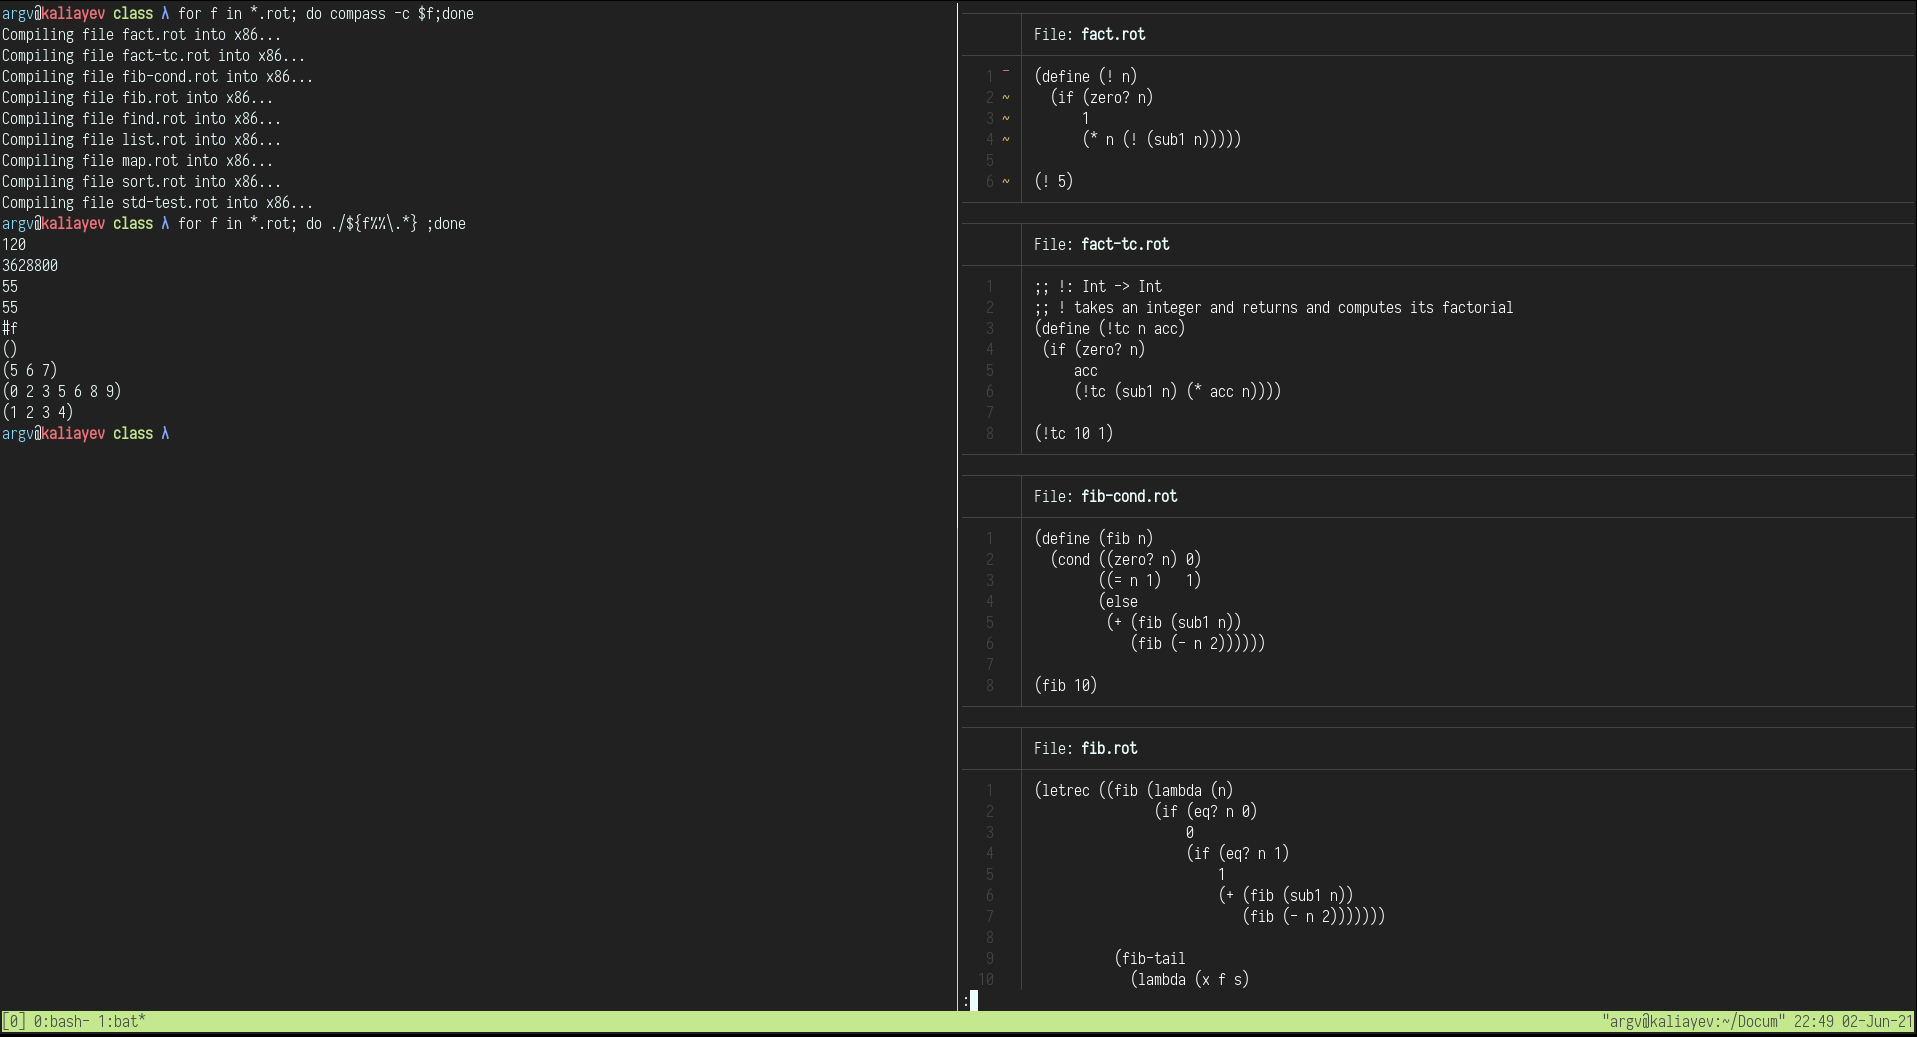
\includegraphics[width=0.8\paperwidth]{figures/ch4/test-run-1}
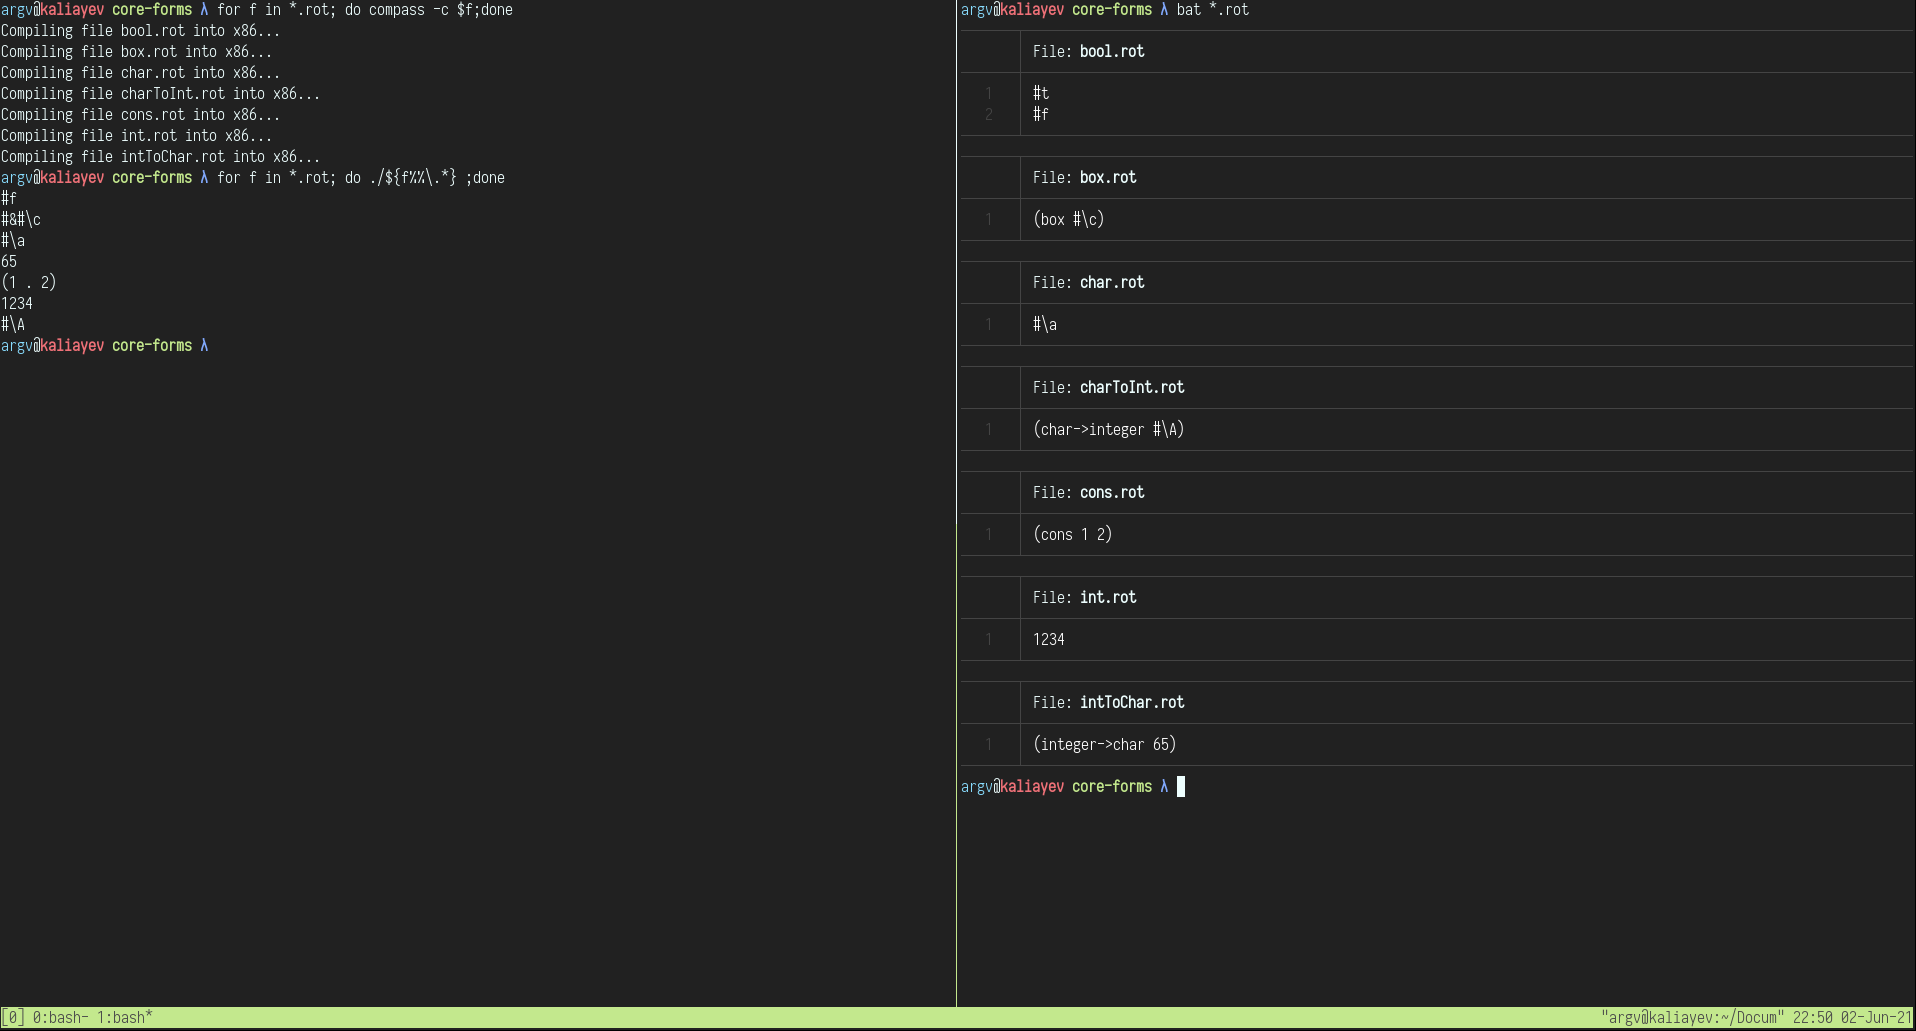
\includegraphics[width=0.8\paperwidth]{figures/ch4/test-run-2}
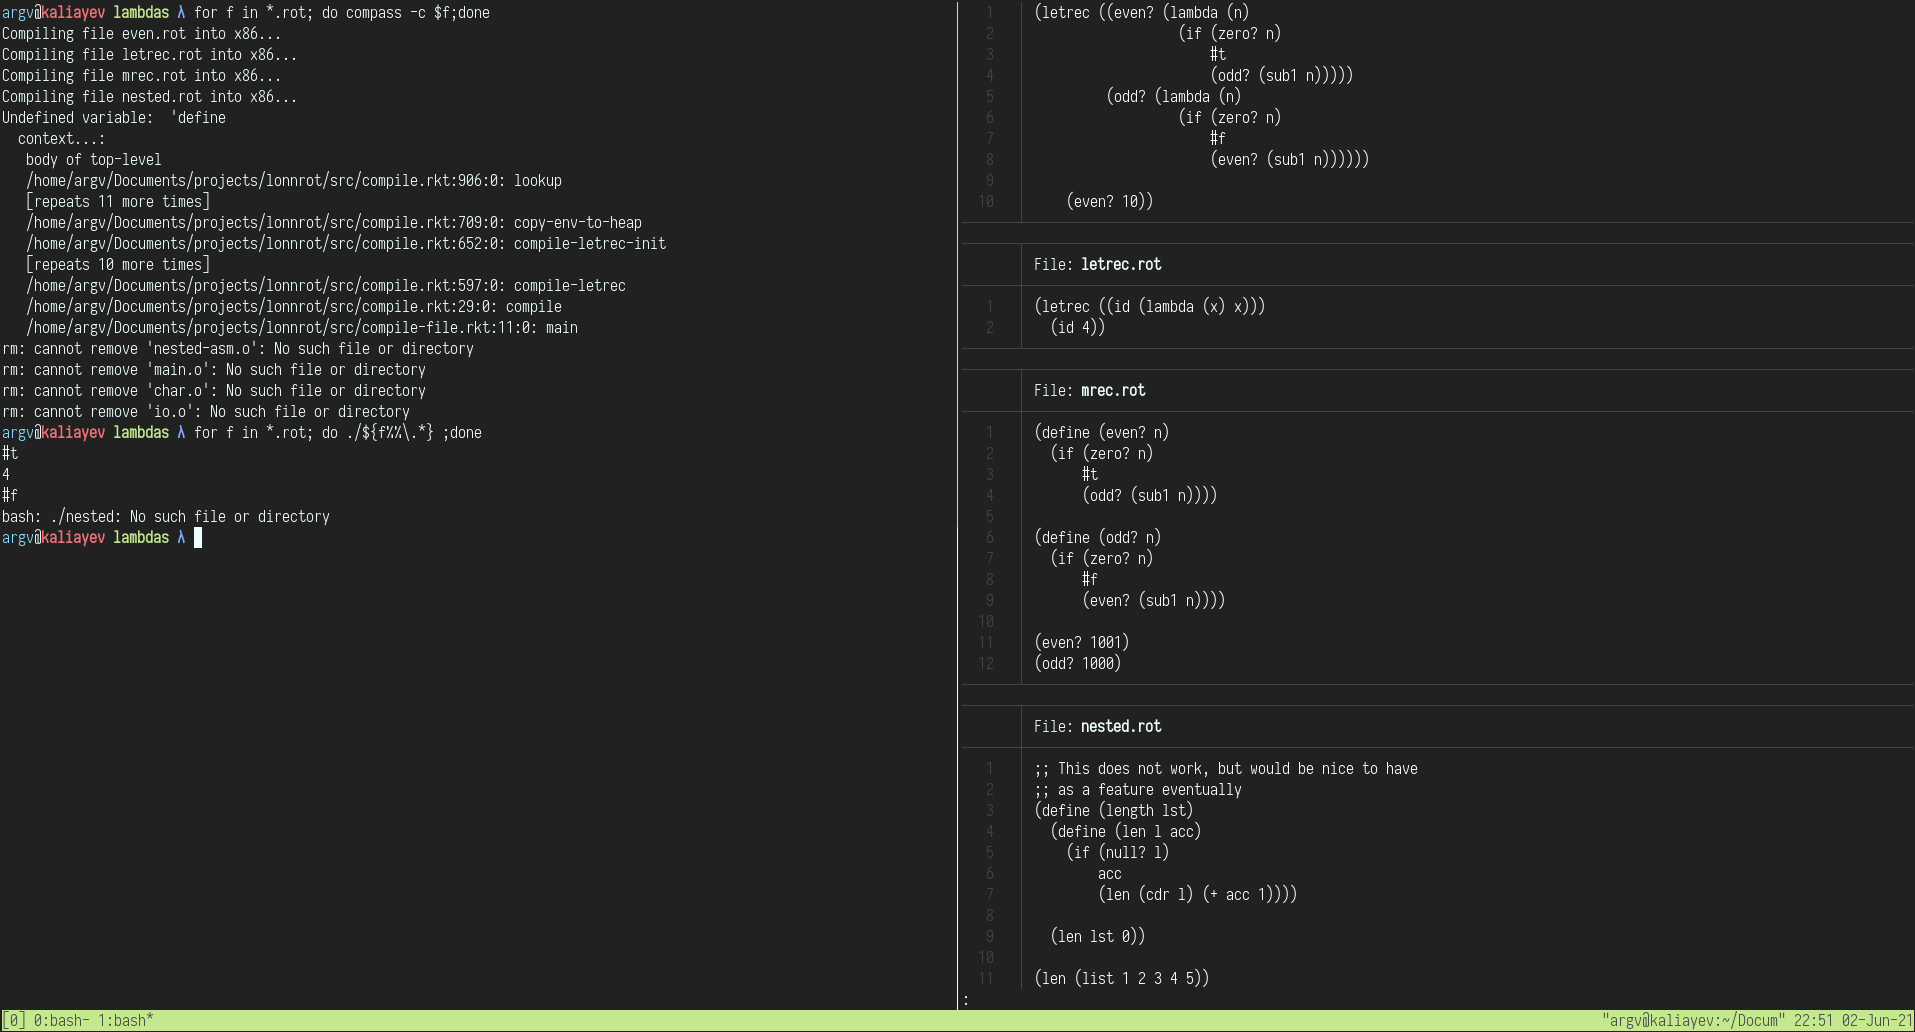
\includegraphics[width=0.8\paperwidth]{figures/ch4/test-run-3}
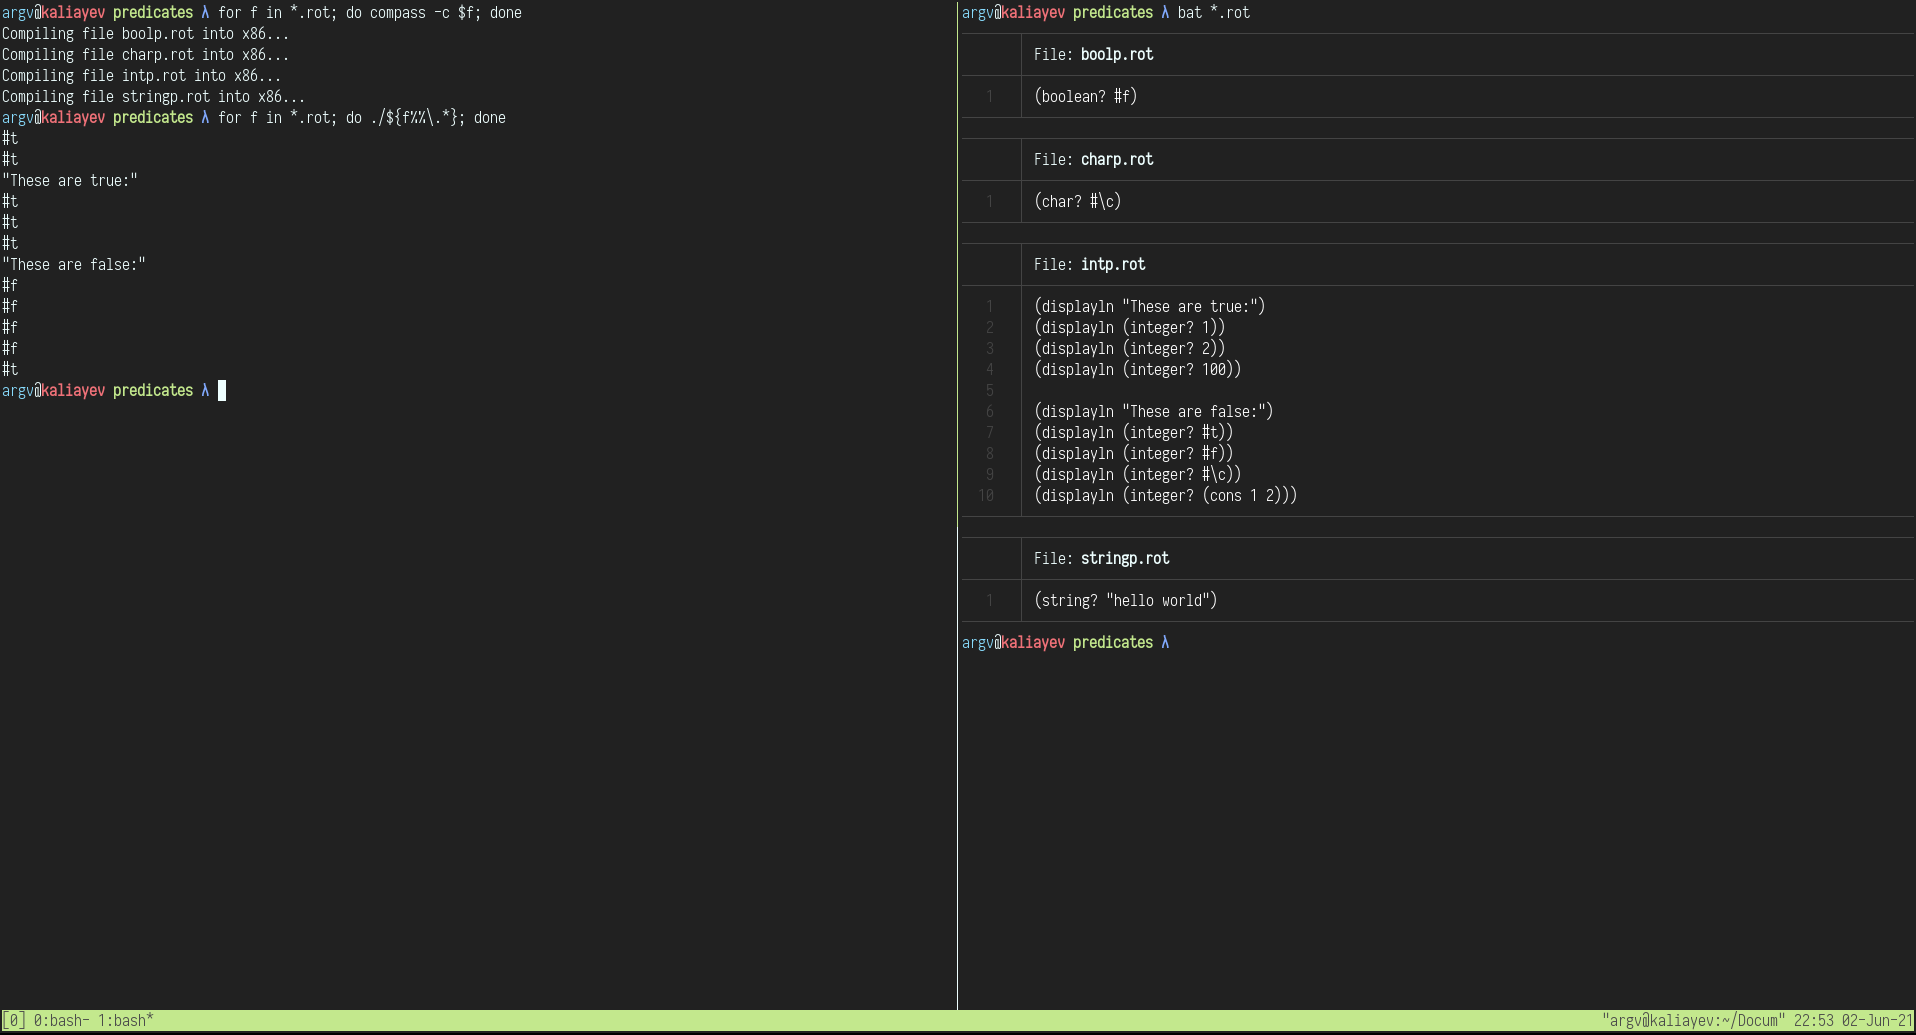
\includegraphics[width=0.8\paperwidth]{figures/ch4/test-run-4}
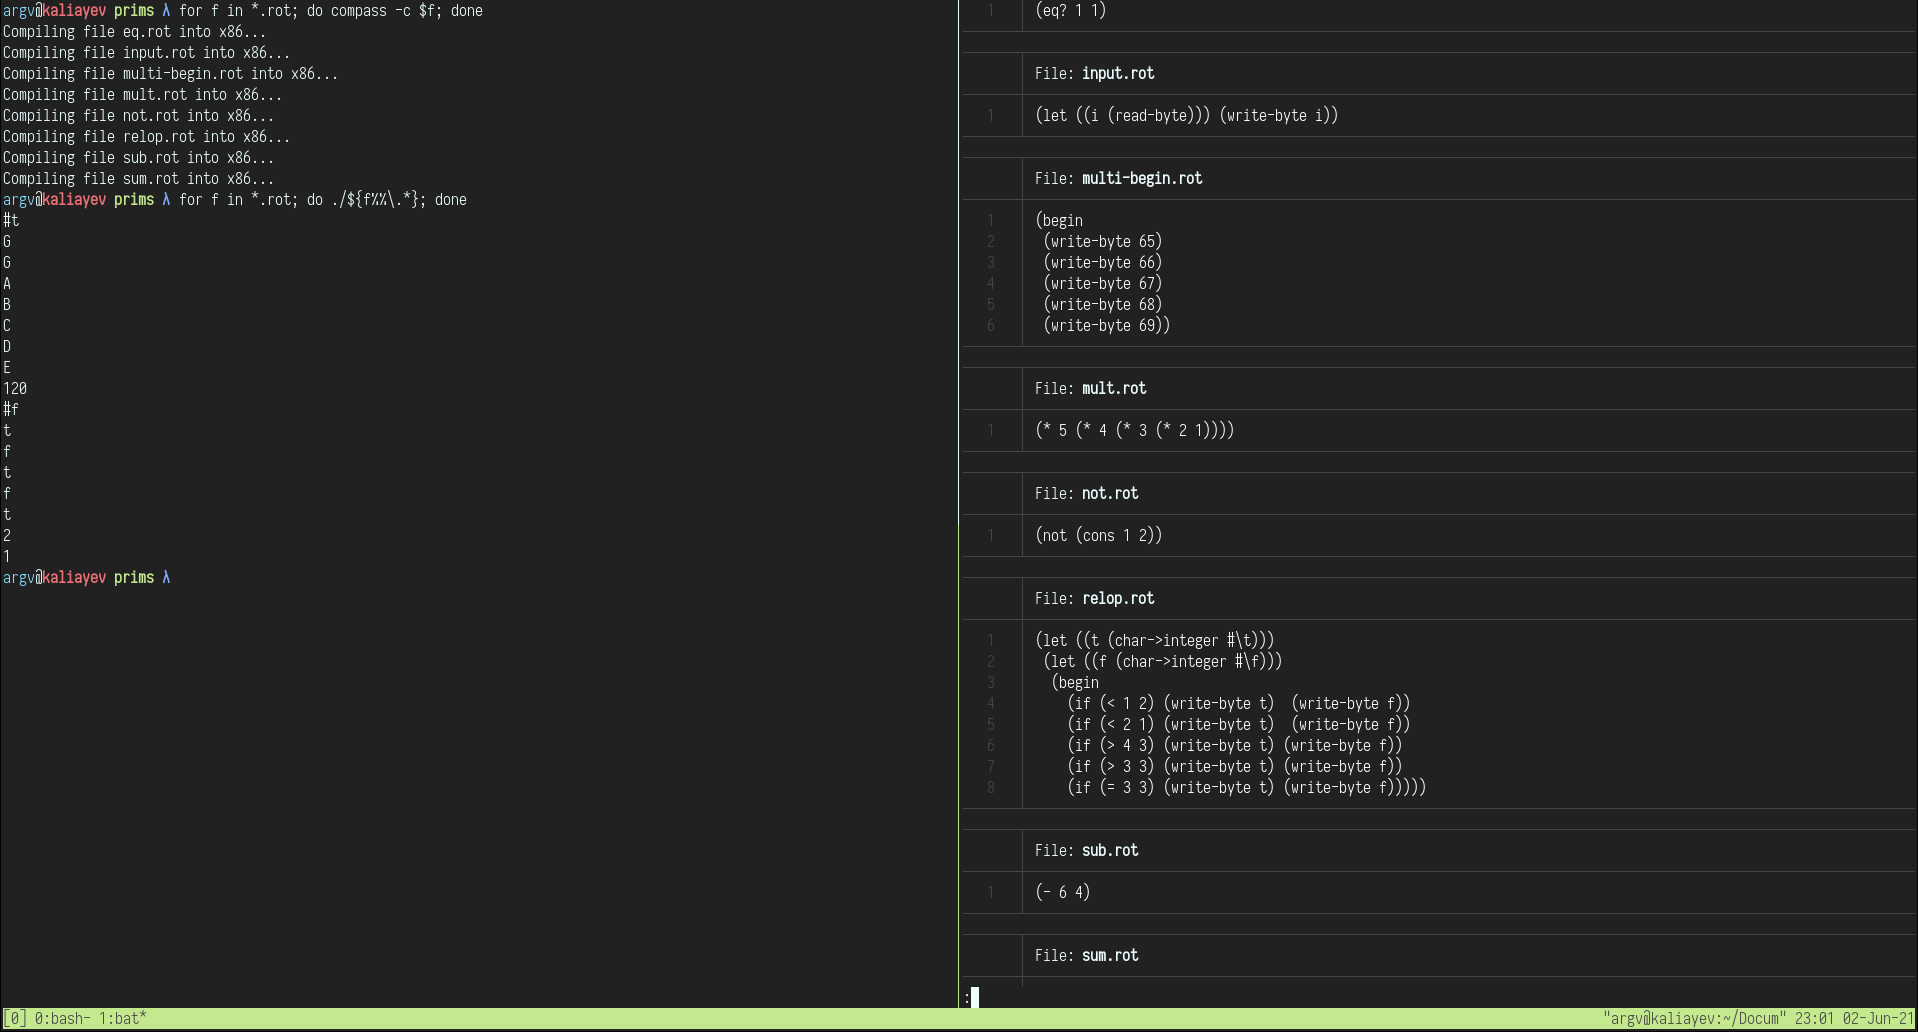
\includegraphics[width=0.8\paperwidth]{figures/ch4/test-run-5}
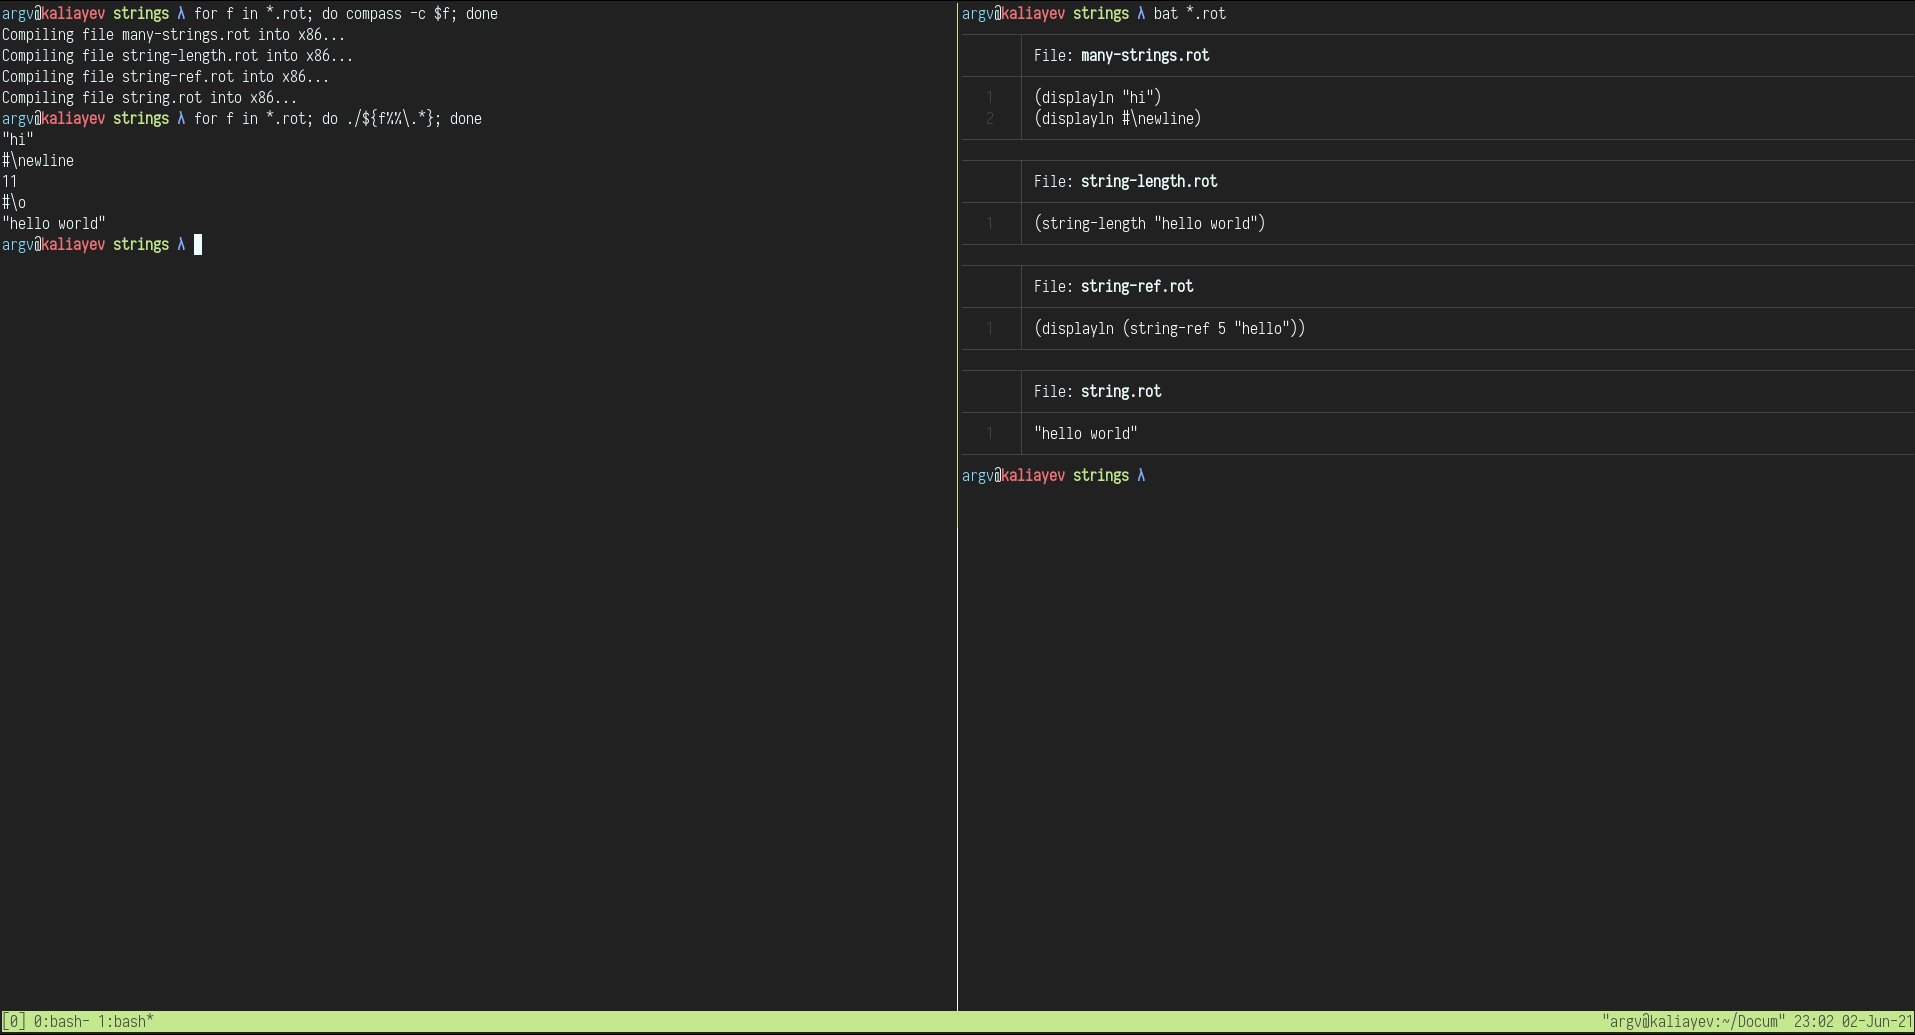
\includegraphics[width=0.8\paperwidth]{figures/ch4/test-run-6}

\clearpage

%chapter 5
%\chapter{Fixed Points, Categorically}\label{ch:categorytheory}

\epigraph{When you see the same beautiful idea pop up everywhere, you begin to think that it is pointing to some deeper truth you haven't yet grasped.}{\textit{Francis Su \cite{su2020}}}

\newthought{Chapter \ref{ch:introduction} motivated}  the investigation of eigenvectors of reduced densities by drawing an analogy with formal concepts---an analogy that was revisited in Section \ref{sec:evectsFCA}. This chapter aims to put that analogy on firmer categorical ground. To do so, we will introduce a \textit{third} construction---a categorical one---that is parallel to both formal concepts and eigenvectors. The category theory will specialize to give formal concepts in a certain case. It will not specialize to the linear algebra, but there is a clear, common categorical thread connecting them, which will be discussed at the end of the chapter.
  \marginnote{This chapter assumes familiarity with the basics of category theory (categories, functors, natural transformations, (co)limits, and adjunctions), though I'll occasionally provide extra commentary for interested readers. For thorough introductions, see \cite{riehl2017category, leinster2014basic, awodey2010category,mac2013categories,spivak2014category, fong2019invitation}. For a lighter treatment of the basics of category theory, see the articles on Math3ma, under the ``Category Theory'' tag \cite{math3ma}. }
 %\tai{``What if we replace probabilities with \textit{possibilities?}''}

Here is an overview of the ideas to come. We will consider three familiar mathematical objects: a vector space with basis set $X$, the power set of a set $X$, and the category of presheaves on a small category $\C$.
\[\mathbb{C}^X \qquad 2^X \qquad \mathsf{Set}^{\C^{\op}}\]
These three objects are related in that all are ``free'' in a sense that can be made precise. Moreover, all three fit into a construction that is strikingly similar to that featured in Chapter \ref{ch:introduction}. To recall, any matrix $M$ corresponds to a function $M\colon X\times Y\to \mathbb{C}$ where $X$ and $Y$ are finite sets. The matrix represents a linear map  $M\colon \mathbb{C}^X\to \mathbb{C}^Y$, which has an adjoint going in the other direction $M^\dagger \colon \mathbb{C}^Y\to\mathbb{C}^X$. The eigenvectors of $M^\dagger M$ and $MM^\dagger$ capture interesting  information about the values $M(i,j)$, especially when they determine a probability distribution on $X\times Y.$ Interestingly, a nearly identical story holds when the complex numbers $\mathbb{C}$ are exchanged for the poset $2$ of \textit{truth values}  (which we define later) or for the category $\mathsf{Set}$. In this chapter we will carefully unwind this claim. 
  \marginnote{Recall that an \emph{adjunction} consists of a pair of functors $\adj{F}{\C}{\D}{G}$ such that there is a natural isomorphism of hom sets \[\C(Fc,d)\cong \D(c,Gd)\] for all objects $c$ in $\C$ and $d$ in $\D$. Equivalently, an adjunction consists of functors $F$ and $G$ together with natural transformations $\eta\colon \id_\C\Rightarrow GF$, called the \emph{unit}, and $\epsilon\colon FG\Rightarrow \id_\D$, called the \emph{counit}, such that the following diagrams commute
  \[
  \begin{tikzcd}[ampersand replacement =\&]
  F \arrow[r, "F\circ\eta", Rightarrow] \arrow[rd, "\id_F"', Rightarrow] \& FGF \arrow[d, "\epsilon \circ F", Rightarrow] \&  \& G \arrow[r, "\eta\circ G", Rightarrow] \arrow[rd, "\id_G"', Rightarrow] \& GFG \arrow[d, "G\circ \epsilon", Rightarrow] \\  \& F                               \&  \&  \& G           
  \end{tikzcd}
  \]
  Here $F\circ \eta$ denotes the natural transformation whose components are of the form $F(\eta_c)\colon F(c)\to FGF(c),$ for each object $c$ in $\C$, and similarly for the others.}

We start in Section \ref{sec:5_LA} by recalling the universal property of a free vector space on a set and will use it to recast the elementary linear algebra of Section \ref{sec:ch1_linalg} in a categorical light. Section \ref{sec:5_CT} discusses another free object with a very similar universal property: the free (co)completion of a category. Unwinding the theory, one finds a number of strong analogies with linear algebra and a clear dictionary between the two worlds. In particular, we will see that categorical version of a matrix $M\colon X\times Y\to\mathbb{C}$ is a functor $R\colon \C^{\op}\times\D\to\mathsf{Set}$; the categorical version of adjoint linear maps $\mathbb{C}^X\rightleftarrows \mathbb{C}^Y$ is an adjunction between (co)presheaf categories $\mathsf{Set}^{\C^{\op}}\rightleftarrows (\mathsf{Set}^\D)^{\op}$; and the categorical version of eigenvectors is a generalized \textit{Isbell completion}. Section \ref{sec:5_FCA} specializes this to the setting of \textit{enriched category theory} by replacing $\mathsf{Set}$ with the poset (category) of truth values $2$. A functor is then a relation $R\colon X\times Y\to 2$; the free (co)completion of a set, viewed as a discrete category, is the free join/meet semilattice on that set; the adjunction between (co)presheaf categories becomes an adjunction of join/meet-preserving maps $2^{X^{\op}}\rightleftarrows (2^Y)^{\op}$; and the generalized Isbell completion gives formal concepts.
\begin{fullwidth}
\begin{center}
\begin{table}[h!]
\begin{tabular}{@{}c|c|c@{}}
\toprule
\textbf{Section \ref{sec:5_LA}} & \textbf{Section \ref{sec:5_CT}} & \textbf{Section \ref{sec:5_FCA}} \\
\midrule
\textsc{linear algebra} & \textsc{category theory} & \textsc{enriched category theory} \\
eigenvectors of reduced densities & generalized Isbell completion & formal concepts\\
\bottomrule
\end{tabular}
\end{table}
\end{center}
\end{fullwidth}

Sections \ref{sec:5_LA}, \ref{sec:5_CT}, and \ref{sec:5_FCA} are meant to feel repetitious. All three are essentially the same story told in different contexts, the motif being that \textit{fixed points of the composition of a morphism with its ``adjoint'' are interesting.} Section \ref{sec:5behind} closes with a remark on the category theory that summarizes this. Here's a quick note on notation. As seen already, sans serif is used for categories $\C$. Also $\C(c,c')$ is used to denote the hom set of morphisms from an object $c$ to an object $c'$ in $\C$. Given categories $\C$ and $\D$, a pair of adjoint functors will be denoted by $\adj{F}{\C}{\D}{G}$ or by $F\dashv G.$



\section{Revisiting Eigenvectors}\label{sec:5_LA}
The motivating construction was already presented in Section \ref{sec:ch1_linalg}, but think of that as the appetizer. In this section, we revisit the elementary linear algebra, this time being mindful of the category theory behind the scenes. \marginnote{I gratefully acknowledge Simon Willerton for his clear exposition on this topic. Indeed, this section---and much of this chapter---was inspired by the excellent writings in \cite{willerton2013} as well as the companion articles \cite{willerton2013b,willerton2014, willerton2015legendrefenchel}.} To start, let $\mathsf{Vect}$ be the category of complex vector spaces and linear transformations, and let $\mathsf{Set}$ be the category of sets and functions. There is a free-forgetful adjunction
\[\adj{U}{\mathsf{Vect}}{\mathsf{Set}}{F}.\]
The functor $U\colon \mathsf{Vect}\to\mathsf{Set}$ associates to any vector space $V$ its underlying set $UV$. The functor $F\colon \mathsf{Set}\to\mathsf{Vect}$ associates to a set $X$ the free vector space $FX$ on $X$. It is ``free'' in that the unit natural transformation $\eta\colon \id_{\mathsf{Set}}\Longrightarrow UF$ of this adjunction fits into the following familiar universal property.

\begin{UP_vect} The \textit{free vector space on a set $X$} is a vector space $FX$ with the property that for any vector space $W$ and for any function $f\colon X\to UW$ there is a unique linear map $\hat f\colon FX\to W$ so that the following diagram commutes
\[
  \begin{tikzcd}
  UFX \arrow[r, "U\hat f", dashed]                  & UW \\
  X \arrow[ru, "f"'] \arrow[u, "\eta_X"] &   
  \end{tikzcd}
\]
\end{UP_vect}
\noindent Concretely, $FX$ is the vector space whose basis is $X$. A vector in $FX$ is then a complex-valued function $v$ on $X$ with the property that $v(x)\neq 0$ for finitely many $x\in X$. The formal sum
\begin{equation}\label{eq:LA_yoneda}
|v\>:=\sum_x v(x)x
\end{equation}
is then guaranteed to be finite and may be thought of as the vector $|v\>$. If $X$ is finite, then vectors in $FX$ may be identified with \textit{all} functions from $X$. In either case, the function $\eta_X$ associates to an element $x\in X$ the independent basis vector $|x\rangle$, and the space $FX$ is sometimes denoted $\mathbb{C}^X$. On any vector $|v\>=\sum_x v(x) |x\>$ in $FX$ the unique lift of any function $f\colon X\to UW$ is defined by
\begin{equation}\label{eq:LA_lift}
\hat f|v\>=\sum_xv(x)f(x).
\end{equation}
Oftentimes, the $U$s are omitted from the diagram and one sees the following.
\[
  \begin{tikzcd}
  \mathbb{C}^X \arrow[r, "\hat f", dashed]                  & W \\
  X \arrow[ru, "f"'] \arrow[u, "\eta_X"] &   
  \end{tikzcd}
\]
But this is not the best practice. The above diagram is not in the correct---or in any!---category. For example, the domain of $f\colon X\to W$ is a set while its codomain is a vector space. The diagrams in Takeaway  \ref{takeaway:LA} also suffered from this ambiguity. Going forward, let's avoid this imprecision. Instead we'll always have in mind the adjunction $\adj{U}{\mathsf{Vect}}{\mathsf{Set}}{F}$ and insert a ``$U$'' where appropriate. Let's also avoid writing ``$FX=\mathbb{C}^X$.'' As noted earlier, vectors in $FX$ may be identified with finitely supported functions $X\to \mathbb{C}$, which explains the convenient exponential notation $\mathbb{C}^X$. But we must be careful. The phrase ``a function $X\to \mathbb{C}$'' has the same problem mentioned above.  On one hand, $X$ is a set; on the other hand, $\mathbb{C}$ is a vector space. An arrow $X\to \mathbb{C}$ is not a morphism in any category, and the exponential $\mathbb{C}^X$ of a vector space by a set is not an object in any category. Rather, here's the better observation: the \textit{underlying set} of the free vector space on $X$ coincides with functions $X\to U\mathbb{C}$. This is summarized in the following takeaway.
\begin{takeaway}\label{takeaway:5LA} Given the free-forgetful adjunction $\adj{U}{\mathsf{Vect}}{\mathsf{Set}}{F},$ the free vector space $FX$ on a set $X$ has the property that
  \begin{equation}\label{eq:EforLA}
  UFX=U\mathbb{C}^X,
  \end{equation}
where $U\mathbb{C}^X$ denotes the set of ``finite'' functions $X\to U\mathbb{C}$, which is all function if $X$ is finite or finitely-supported functions otherwise. In short, the adjunction $F\dashv U$ has the property that there is a special object in $\mathsf{Vect}$, namely $\mathbb{C}$, such that \textit{all} free vector spaces are, in some sense, built up from it.
\end{takeaway}

Now we are close to rediscovering Takeaway \ref{takeaway:LA} in Chapter \ref{ch:introduction}. Suppose $X$ and $Y$ are finite sets and consider any function $M\colon X\times Y\to U\mathbb{C}$. The category of sets is Cartesian closed, and so we have a product-hom adjunction and hence the following bijections.
  \marginnote[2cm]{A category $\C$ is called \emph{Cartesian closed} if for every pair of objects $x$ and $z$ there is an object $z^x$ in $\C$ so that for all objects $y$ there is a natural bijection \[\C(x\times y,z)\cong \C(y,z^x)\] The object $z^x$ is called the \emph{internal hom} and should be thought of as a $\C$'s worth of morphisms from $x$ to $z$.}
\[
  \begin{tikzcd}
  {\mathsf{Set}(X,U\mathbb{C}^Y)} & \cong & {\mathsf{Set}(X\times Y,U\mathbb{C})}                 & \cong & {\mathsf{Set}(Y,U\mathbb{C}^X)} \\[-20pt]
  \alpha             &       & M \arrow[rr, maps to] \arrow[ll, maps to] &       & \beta            
  \end{tikzcd}
\]
Under this adjunction, the function $\alpha\colon X\to U\mathbb{C}^Y$ is defined on each $x\in X$ by $\alpha x(y)= M(x,y)$. Likewise define the function $\beta\colon Y\to U\mathbb{C}^X$ on each $y\in Y$ by $\beta y(x)=\overline{M(x,y)}$. By the universal property for vector spaces, $\alpha$ lifts uniquely to a linear map $M\colon FX\to FY$, and $\beta$ lifts uniquely to a linear map $M^\dagger \colon FY\to FX$ so that the following diagrams commute.
\begin{equation}\label{diagrams:correctlifts_LA}
  \begin{tikzcd}
  U\mathbb{C}^X \arrow[r, "UM", dashed]         & U\mathbb{C}^Y && U\mathbb{C}^Y \arrow[r, "UM^\dagger ", dashed]         & U\mathbb{C}^X \\
  X \arrow[ru, "\alpha"'] \arrow[u, hook] &     && Y \arrow[u, hook] \arrow[ru, "\beta"'] &    
  \end{tikzcd}
\end{equation}
What's more, $M$ and $M^\dagger$ are linear adjoints so that
\begin{equation}\label{eq5:adjoint}
\langle Mv,w\rangle = \langle v,M^\dagger w\rangle \qquad \text{for all $v\in FX$ and $w\in FY$.}
\end{equation}
If we drop the ``$U$s'' from the diagrams, then we recover the contents of Takeaway \ref{takeaway:LA}. When the function $M\colon X\times Y\to U\mathbb{C}$ further satisfies the condition that $\sum_{x,y}|M(x,y)|^2=1$, then it represents a pure quantum state in $FX\otimes FY$, and we've shown in detail in Chapter \ref{ch:probability} that the eigenvectors of the reduced density operators $MM^\dagger $ and $M^\dagger M$ harness valuable information from that state.  

These ideas, though elementary, set the stage for the remainder of this chapter. Here are the key points to have in mind. We started with the free-forgetful adjunction $\adj{U}{\mathsf{Vect}}{\mathsf{Set}}{F}$ and observed that $\mathsf{Vect}$ contains a special object, namely $\mathbb{C}$, with the property that the free space $FX$ on a set $X$ always ``looks like'' functions from $X$ to $U\mathbb{C}$. As a result, every  function $X\times Y\to U\mathbb{C}$ gives rise to a pair of adjoint maps $\adj{M}{FX}{FY}{M^\dagger}$, whose composites $M^\dagger M$ and $MM^\dagger$ have interesting fixed points.\sidenote{That is, they have interesting \textit{eigenvectors}. So we may restate our claim is, ``The one-dimensional invariant subspaces of $M^\dagger M$ and $MM^\dagger$ are interesting.''} This very same template will reappear in Section \ref{sec:5_CT} and again in Section \ref{sec:5_FCA}. More precisely, the idea that ``fixed points of a map with its adjoint are interesting'' is strikingly similar to a known scenario in category theory---there is nearly a word-for-word analogy between the two.  Even better, the categorical version recovers the formal concept construction in Section \ref{sec:ch1_FCA} as a special case. Let's discuss this category theory now.


\section{Free (Co)Completions}\label{sec:5_CT}
%Briefly introduce limits/colimits first, a la Math3ma abridged?

To construct the free vector space on a set $X$, we added all formal sums of elements in $X$. Category theory generalizes sums through \emph{colimits}, and it generalizes multiplication through \emph{limits}. We refer to any basic text for the formal definitions \cite{riehl2017category}. But here are three \textit{informal} things to know.
  \begin{enumerate}
    \item \textbf{Intuition.} Colimits and limits subsume many constructions in mathematics. Unions of sets and joins in a poset are two examples of colimits. Cartesian products of sets and meets in a poset are two examples of limits. Informally, colimits have a ``glue-y'' feel to them, whereas limits have an ``equation-y'' feel to them.

    \item \textbf{Vocabulary.} One always takes the (co)limit \textit{of} something. That ``something'' is a \emph{diagram} in a category $\C$, which is synonymous with a functor whose codomain is $\C$. The diagram is called \emph{small} if the domain of the functor is a small category. (See the next bullet.) A category is called \emph{cocomplete} if it contains  colimits of all small diagrams; it is called \emph{complete} if it contains limits of all small diagrams.

    \item \textbf{More Vocabulary.} A category is called \emph{small} if the morphisms of the category form a set. It is called \emph{locally small} if the morphisms between any two objects form a set. As an example, the category with two objects and a single nonidentity arrow $\bullet\to\bullet$ is small and hence locally small, whereas $\mathsf{Set}$ is locally small but not small.
  \end{enumerate} 

\newthought{As in the linear} algebra of Section \ref{sec:5_LA}, the starting ingredient for this section is an adjunction. Let $\mathsf{CAT}$ denote the category whose objects are locally small categories and whose morphisms are functors. Let $\mathsf{CocompCAT}$ denote the category of locally small cocomplete categories and cocontinuous functors between them.\sidenote{A functor is said to be \emph{cocontinuous} if it takes colimits to colimits.} Both $\mathsf{CAT}$ and $\mathsf{CocompCAT}$ are actually 2-categories; that is, there are morphisms (natural transformations) between the morphisms (functors). There is a free-forgetful ``adjunction'' between these 2-categories.
\[\adj{U}{\mathsf{CocompCAT}}{\mathsf{CAT}}{F}.\]
The functor $U\colon \mathsf{CocompCAT}\to \mathsf{CAT}$ associates to any locally small cocomplete category $\D$ its underlying category $U\D$. The functor $F\colon \mathsf{CAT}\to\mathsf{CocompCAT}$ associates to a locally small category $\C$ the \emph{free cocomplete category} $F\C$ on $\C$. The setup here isn't quite an adjunction in the usual sense, as 2-categorical considerations prevent it from being so. Instead, it is called a \emph{biadjunction}, which is the appropriate notion of adjunctions in this higher-categorical setting. But here's the main idea for us: just as every set gives rise to a free vector space, so every category $\C$ gives rise to a free cocomplete category $F\C$ \cite{Day_2007,kelly200,nlab:free_cocompletion}. Crucially, $F\C$ is free in that unit $\eta\colon \id_{\mathsf{CAT}}\Longrightarrow UF$ of the biadjunction has the following universal property.


\begin{UP_cocomplete}The \textit{free cocompletion of a category $\C$} is a cocomplete category $F\C$ with the property that for any other cocomplete category $\D$ and for any functor $f\colon \C\to U\D$, there is a unique cocontinuous functor $\hat f\colon F\C \to \mathsf{D}$ so that the following diagram commutes up to natural isomorphism.
\[
  \begin{tikzcd}
  UF\C \arrow[r, "U\hat f", dashed] & U\mathsf{D} \\
  \C \arrow[ru, "f"'] \arrow[u,"\eta_\C"]                 &   
  \end{tikzcd}
\]
\end{UP_cocomplete}
Let's unwind this statement. First, the category $F\C$ has a familiar construction. If $\C$ is small, then its free cocompletion is the category of all contravariant functors from $\C$ to $\mathsf{Set}$, also called \emph{presheaves} \cite{Day_2007}. It is typically written as\sidenote{Every category $\C$ has an \emph{opposite category} $\C^{\op}$ whose objects are the same as the objects in $\C$. A morphism $c\to c'$ in $\C^{\op}$ is defined to be a morphism $c'\to c$ in $\C$. As a result, for any category $\D$, a contravariant functor $\C\to \D$ is a functor $\C^{\op}\to \D$.}
\[F\C=\mathsf{Set}^{\C^{\op}}.\]
If the category $\C$ is \textit{not} small, then the construction of $F\C$ needs a minor adjustment, which will be explained shortly. But first, know that the unit $\eta_\C\colon \C\to UF\C$ of the biadjunction is the \emph{Yoneda embedding} $c\mapsto \C(-,c)$. Oftentimes the ``$U$''s are omitted from the diagram and one typically sees
\[
  \begin{tikzcd}
  \mathsf{Set}^{\C^{\op}}\arrow[r, "\hat f", dashed] & \mathsf{D} \\
  \C \arrow[ru, "f"'] \arrow[u,"\eta_\C"]                 &   
  \end{tikzcd}
\]
But let's be careful to insert a ``$U$'' where appropriate. In particular---and for reasons explained below---it's better not to write ``$F\C=\mathsf{Set}^{\C^{\op}}$,'' even though the notation may be familiar. We will suggest a better observation in Takeaway \ref{takeaway:5CT} later on. 

Now, how are we to understand the free cocompletion $F\C$ when $\C$ is a locally small (possibly large) category? Size issues prevent the presheaf category from being its free cocompletion, so a minor adjustment must be made. To motivate the idea, it will help to think back to the familiar linear algebra of Section \ref{sec:5_LA}. Recall that the free vector space on a set $X$ does not coincide with \textit{all} functions $X\to U\mathbb{C}$ but rather only those functions with finite support. In a completely analogous way, if $\C$ is not small, then its free cocompletion does not coincide with \textit{all} functors $\mathsf{C}^{\op}\to\mathsf{Set}$ but rather only those functors that are ``finite,'' or more precisely, \emph{small}. (Intuitively, a presheaf is said to be small if it can be written as a small colimit of representable functors.) For a precise definition and a thorough treatment of these ideas see \cite{Day_2007}.

Continuing to unwind the universal property, how should we understand the unique cocontinuous extension $\hat f$ along the Yoneda embedding? To aid intuition, we draw another comparison with linear algebra. Recall from the universal property for vector spaces that any function on a set $X$ lifts to a linear map on the free vector space on $X$ that agrees with the function on basis elements in $X$. Simply put, the lift is a \textit{linear extension} of the function. In a completely analogous way, the universal property above says that any functor $f\colon \C\to U\D$ has a ``cocontinuous extension'' $\hat f\colon F\C\to \D$ that agrees with $f$ on \emph{representable functors}, which are very much like basis vectors of the presheaf category $\mathsf{Set}^{\C^{\op}}$.\marginnote{``The representables are the prime numbers of presheaves.'' \cite{leinster2014basic}} More formally, \textit{any presheaf $V\colon \C^{\op}\to \mathsf{Set}$ is a colimit of representable functors}, which are functors of the form $\mathsf{C}(-,c)\colon \C^{\op}\to\mathsf{Set}$ for some object $c$ in $\C$ \cite[Theorem 6.5.8]{riehl2017category}, \cite[Theorem 6.2.17]{leinster2014basic}. There are a few ways to express this statement notationally. Here's one way that uses notation that we have not defined, but which is very suggestive \cite[Proposition 2.2.1]{loregian2015coend}.\sidenote{See also \cite[Proposition 2.2]{nlab:co-yoneda_lemma} and \cite[Section 2]{nlab:free_cocompletion}.} For any presheaf $V$, one has
\begin{equation}\label{eq:CT_yoneda}
V\cong \int^{c\in\C} \C(-,c)\cdot Vc,
\end{equation}
and the lift $\hat f$ in the universal property is then defined by
\begin{equation}\label{eq:CT_lift}
\hat{f}V:= \int^{c\in\C} fc \cdot Vc.
\end{equation}
The integral $\int^{c\in \C}$ is a type of a colimit called a \textit{coend}. The dot $\cdot$ is called a \textit{copower}, and the expression $\C(-,c)\cdot Xc$ denotes the $Xc$-indexed coproduct of the hom-functor $\C(-,c)$ with itself, and similarly for $fc\cdot Vc$. The particulars are not needed here, but we mention this simply to point out the similarities between Equation (\ref{eq:CT_yoneda}) and Equation (\ref{eq:LA_yoneda}),
\[
\begin{array}{c@{\hspace{3ex}}|@{\hspace{3ex}}c}
|v\>=\displaystyle\sum_{x\in X} v(x)|x\>
&
V\cong \displaystyle\int^{c\in\C} \C(-,c)\cdot Vc
\end{array} 
\]
and between Equation (\ref{eq:LA_lift}) and Equation (\ref{eq:CT_lift}).
\[
\begin{array}{c@{\hspace{3ex}}|@{\hspace{3ex}}c}
\hat f|v\>=\displaystyle\sum_{x\in X}v(x)f(x)
&
\hat{f}V= \displaystyle\int^{c\in\C} fc \cdot Vc
\end{array} 
\]
The analogy is clear: presheaves are \textit{like} vectors, representable functors are \textit{like} basis vectors, colimits are \textit{like} sums, cocontinuous functors are \textit{like} linear maps, and so on.\sidenote[][-3cm]{Here's yet another analogy. If $M$ is an $n\times m$ matrix and $N$ is an $m\times p$ matrix, then $MN$ is an $n\times p$ matrix whose $ij$th entry is obtained by ``tracing out'' a common index $\sum_k M_{ik}N_{kj}$. The categorical version of a matrix $X\times Y\to U\mathbb{C}$ is a \textit{profunctor}, which is the name given to a functor of the form $\C^{\op}\times D\to \mathsf{Set}$.  The composition of two profuctors $F\colon \C^{\op}\times \D\to\mathsf{Set}$ and $G\colon \D^{\op}\times \E\to\mathsf{Set}$ is given by a coend, which is a colimit over the common index $FG=\displaystyle \int^{d\in \D}F(-,d)\times G(d,-).$ More generally, one could imagine composing profunctors several variables, which brings to mind tensor contraction. I first learned of this analogy from \cite{Kissinger2011}.} 


\newthought{In summary}, the free cocompletion $F\C$ of a category $\C$ is very much like the free vector space $FX$ on a set $X$. As suggested above, it's better not to use the notation ``$F\C=\mathsf{Set}^{\C^{\op}}.''$ The category $\mathsf{Set}$ has many nice properties, one of them being that it is cocomplete. Since an arbitrary category $\C$ may \textit{not} be cocomplete, an arrow $\C^{\op}\to \mathsf{Set}$ is not well-typed. Instead, it's better to say that a presheaf is a functor from $\C^{\op}$ to the \textit{underlying category} of the cocomplete category $\mathsf{Set}$, and that the \textit{underlying category} of the free cocompletion $F\C$ coincides with these presheaves. This is summarized in the takeaway below. Compare it with the linear algebra in Takeaway \ref{takeaway:5LA}.

\begin{takeaway}\label{takeaway:5CT}
Given the free-forgetful biadjunction $\adj{U}{\mathsf{CocompCAT}}{\mathsf{CAT}}{F}$, the free cocompletion $F\C$ of a category $\C$ has the property that
\begin{equation}
UF\C=U\mathsf{Set}^{\C^{\op}},
\end{equation}
where $U\mathsf{Set}^{\C^{\op}}$ denotes the category of ``small'' presheaves $\C^{\op}\to U\mathsf{Set}$, namely all presheaves if $\C$ is small or small presheaves otherwise. In short, the adjunction $F\dashv U$ has the property that there is a special object in $\mathsf{CocompCAT}$, namely $\mathsf{Set}$, such that all free cocomplete categories are, in some sense, built up from it.
\end{takeaway}

As expected, there is a dual discussion obtained by ``reversing all the arrows.'' It's worth mentioning briefly. Let $\mathsf{CompCAT}$ denote the 2-category of locally small complete categories, continuous functors,\sidenote{A functor is said to be \emph{continuous} if it takes limits to limits.} and natural transformations between them. There is a free-forgetful biadjunction 
\[\adj{U}{\mathsf{CompCAT}}{\mathsf{CAT}}{\bar F}.\]
The functor $U\colon \mathsf{CompCAT}\to \mathsf{CAT}$ associates to any complete category $\C$ its underlying category $U\C$. The functor $\bar F\colon \mathsf{CAT}\to\mathsf{CompCAT}$ associates to a category $\C$ the \emph{free complete category} $\bar F\C$ on $\C$. It is free in that the unit $\eta\colon \id_{\mathsf{CAT}}\Longrightarrow U\bar F$ of this biadjunction satisfies the following universal property.

\begin{UP_complete}The \textit{free completion of a category $\C$} is a complete category $\bar F\C$ with the property that for any complete category $\D$ and for any functor $g\colon \C\to U\D$, there is a unique continuous functor $\hat g\colon \bar F\to \D$ so that the following diagram commutes up to natural isomorphism.
\[
  \begin{tikzcd}
  U \bar F\C \arrow[r, "U\hat g", dashed] & U\D \\
  \C \arrow[ru, "g"'] \arrow[u,"\eta_{\C}"]                 &   
  \end{tikzcd}
\]
\end{UP_complete}
\noindent The free completion $\bar F\C$ is constructed as\sidenote{One may find difficulty in locating this explicit statement in the literature since it is a formal consequence of the free cocompletion construction. One place to start is the nLab's article on free completions \cite{nlab:free_completion}.} the opposite category of \textit{co}presheaves on $\C$, typically denoted $(\mathsf{Set}^{\C})^{\op}$. So $\bar F \C$ is the category whose objects are (small) functors $f\colon \C\to U\mathsf{Set}$, and where a morphism between copresheaves $f\to f'$ is a natural transformation going in the other direction $f'\Longrightarrow f.$  In particular, when $\C$ is a small category $\bar F\C$ coincides with \textit{all} copresheaves $\C\to U\mathsf{Set}$. In either case, the free completion of $\C$ has the property that 
\[ U\bar F \C = (U\mathsf{Set}^{\C})^{\op},\]
where the right-hand side is the category of small (and thus all when $\C$ is small) functors $\C\to U\mathsf{Set}$. The functor $\eta_{\C}\colon \C\to U\bar F\C$ in the universal property is the \textit{dual} Yoneda embedding that sends an object $c\in \C$ to its representable functor $\C(c,-)$, and the unique continuous extension $\hat g$ is defined dually to the unique cocontinuous extension in Equation (\ref{eq:CT_lift}).

%Use the fact that any copresheaf $W$ can be written as a limit of representable functors $W\cong\int_{c\in C} \C(c,-)^{Wc}$, where the notation $\C(c,-)^{Wc}$ is called a \textit{power} and denotes the $Wc$-indexed product of copies of $\C(c,-)$  \tai{(Fosco has them flipped; also weird that he takes copower as product! Maybe omit details? or put in margin since NO ONE ever says this.)}. Perhaps not surprisingly, then, the unique lift $\hat g$ of any functor $g\colon \C\to U\D$ is given by \[\hat gW=\int_{c\in \C} {gc}^{Wc}.\]

\newthought{There is quite} a bit of heavy machinery here, but we won't need to work with it explicitly. We mentioned it simply to call attention to the fact that \textit{there exists} well-developed theory that connects with familiar ideas in linear algebra and---as we'll see in the next section---formal concept analysis. En route to making this connection clearer, let us close with one final remark. Suppose $\C$ is a small category. We have the following two observations.
\begin{description}
\item \textit{The free cocomplete category $F\C$ is not only cocomplete, it is also complete.}

\item \textit{The free complete category $\bar F \C$ is not only complete, it is also cocomplete.}
\end{description}
The reason behind both statements is simple. The category of (contravariant) functors $\C^\to U\mathsf{Set}$ inherits (co)completion from $\mathsf{Set}$, which is both complete and cocomplete. The (co)limit of any diagram of functors $\C^{\op}\to\mathsf{Set}$ is obtained by evaluating them pointwise and then computing the (co)limit in $\mathsf{Set}$. This is analogous to how the set of functions from a set $X\to\mathbb{C}$ inherits a vector space structure from $\mathbb{C}$ by pointwise evaluation. These simple observations lead to our final analogy with linear algebra.\sidenote{The following discussion should be compared with the analogous discussion in Section \ref{sec:5_LA}.}

Let $\D$ be a small category. Any functor $M\colon C^{\op}\times \D\to U\mathsf{Set}$
gives rise to functors $A$ and $B$ on each factor, 
\[
  \begin{tikzcd}
  {\mathsf{Cat}(\C^{\op},U\mathsf{Set}^\D)} & & {\mathsf{Cat}(\C^{\op}\times \D,U\mathsf{Set})}\arrow[ll]\arrow[rr]                 & & {\mathsf{Cat}(\D,U\mathsf{Set}^{\C^{\op}})} \\[-20pt]
  A             &       & M \arrow[rr, maps to] \arrow[ll, maps to] &       & B            
  \end{tikzcd}
\]
Notice that functors $\C^{\op}\to U\mathsf{Set}^\D$ on the left-hand side are in bijection with functors $\C\to (U\mathsf{Set}^\D)^{\op}$. Under this correspondence, the functor $A\colon \C\to (U\mathsf{Set}^\D)^{\op}$ obtained from $M$ is defined on an object $c$ in $\C$ by $Ac(d)=M(c,d)$ for each object $d$ in $\D$. Likewise the functor $B\colon \D\to U\mathsf{Set}^{\C^{\op}}$ is defined on each $d$ by $Bd(c)=M(c,d)$. By the universal property for free cocompletions, $A$ lifts uniquely to a cocontinuous functor $M^*\colon F\C\to \bar F\D$, and by the universal property for free completions, $B$ lifts uniquely to a continuous functor $M_*\colon \bar F\D\to F\C$ so that the following diagrams commute,
\begin{equation}\label{diagrams:correctlifts_CT}
  \begin{tikzcd}
  U\mathsf{Set}^{\C^{\op}} \arrow[r, "UM^*", dashed]         & (U\mathsf{Set}^\D)^{\op} && (U\mathsf{Set}^\D)^{\op} \arrow[r, "UM_*", dashed]         & U\mathsf{Set}^{\C^{\op}} \\
  \C \arrow[ru, "A"'] \arrow[u, hook] &     && \D \arrow[u, hook] \arrow[ru, "B"'] &    
  \end{tikzcd}
\end{equation}
See the excellent exposition in \cite{willerton2013} for explicit expressions for $M^*$ and $M_*$ in the enriched setting, and compare this with the analogous discussion in Section \ref{sec:5_LA} leading up to the two diagrams in (\ref{diagrams:correctlifts_LA}). The climax here is that the functors $M^*$ and $M_*$ are adjoints. That is, there is a natural isomorphism $(\mathsf{Set}^\D)^{\op}(M^*V,W)\cong \mathsf{Set}^{\C^{\op}}(V,M_*W)$ for all presheaves $V$ and copresheaves $W$. Here we have lifted our self-imposed ban on writing $F\C=\mathsf{Set}^{\C^{\op}}$ to call attention to the ``op'' on the left-hand side of the isomorphism. A morphism $M^*V\to W$ in $(\mathsf{Set}^\D)^{\op}$ is a morphism $W\to M^*V$ in $\mathsf{Set}^\D$, and so we may rewrite the correspondence as
\[\mathsf{Set}^\D(W,M^*V)\cong \mathsf{Set}^{\C^{\op}}(V,M_*W).\]
The functors $M_*$ and $M^*$ are thus said to be \textbf{mutually right adjoints} that come with ``unit'' natural transformations  $\eta\colon \id \Longrightarrow M_*M^*$ and $\epsilon \colon \id \Longrightarrow M_*M^*$ \cite[Definition 4.3.1]{riehl2017category}, and their invariant subcategories, or ``fixed points,'' now arise as the topic of interest.\marginnote{Let's say an object $a$ in a category $\C$ is \textit{invariant} under a functor $F\colon\C\to\D$ if there is an isomorphism $a\overset{\cong}{\longrightarrow} Fa.$} Let $\text{Fix}(M_*M^*)$ be the category whose objects are objects $c$ in $\C$ such that the unit $\eta_c\colon c \overset{\cong}{\longrightarrow} M_*M^*c$ is an isomorphism. Likewise, let $\text{Fix}(M^*M_*)$ denote the category hose objects are objects $d$ in $\D$ so that $\epsilon_d\colon d \overset{\cong}{\longrightarrow} M^*M_*d$ is an isomorphism. There is an equivalence of categories\sidenote{This is a standard exercise. Every adjunction restricts to an equivalence of categories in this way.}
\[
\text{Fix}(M_*M^*)\cong
\text{Fix}(M^*M_*)
\] 
and their objects are called the \textbf{nucleus} of $M$. When $\D=\C$ and $M\colon \C^{\op}\times \C\to\mathsf{Set}$ is the hom-functor $\C(-,-)$, the adjunction $M^*\dashv M_*$ is called the \textbf{Isbell adjunction} or Isbell conjugation, and its nucleus is called the \emph{Isbell completion} of $\C$. If $\mathsf{Set}$ is further replaced by the category $2$ of truth values (defined in the next section) and the category $\C$ is a poset $P$, then this recovers the \emph{Dedekind MacNeille completion of $P$}. If $P=\mathbb{Q}$ with the usual ordering, then the Isbell completion gives the completion of $\mathbb{Q}$ by Dedekind cuts. If instead of replacing $\mathsf{Set}$ by $2,$ we were to replace it with $[0,\infty]$ with an appropriate categorical structure, this recovers the \emph{tight span} of a metric space. For more on these constructions see \cite{willerton2015legendrefenchel,pavlovic2012quantitative,isbell1966structure,Lawvere86takingcategories,Elliott2017OnTF,willerton2013tight}. By now we've covered a lot of information in a small amount of space. Here's the takeaway.

%and the category $\text{Fix}(M_*M^*)\cong \text{Fix}(M^*M_*)$ is called the \textbf{Isbell evelope} or \textbf{Isbell completion} of $\C$ \cite{Lawvere86takingcategories}. 

\begin{takeaway}\label{takeaway:5CTa}
Given small categories $\C$ and $\D$, any functor $M\colon \C^{\op}\times \D\to U\mathsf{Set}$ induces two functors $A\colon \C\to U\mathsf{Set}^{\C^{\op}}$ and $B\colon \D\to (U\mathsf{Set}^\D)^{\op}$ that lift to a cocontinuous functor $M^*$ and a continuous functor $M_*$ so that the following diagrams commute.
\begin{equation}\label{diagrams:presheaf_lifts}
  \begin{tikzcd}
  U\mathsf{Set}^{\C^{\op}} \arrow[r, "M^*", dashed]         & (U\mathsf{Set}^{\D})^{\op} && (U\mathsf{Set}^{\D})^{\op} \arrow[r, "M_*", dashed]         & U\mathsf{Set}^{\C^{\op}} \\
  \C \arrow[ru, "A"'] \arrow[u, hook] &     && \D \arrow[u, hook] \arrow[ru, "B"'] &    
  \end{tikzcd}
\end{equation}
Moreover $M^*$ and $M_*$ satisfy
\[\mathsf{Set}^\D(W,M^*V)\cong \mathsf{Set}^{\C^{\op}}(V,M_*W)\]
for all presheaves $V$ in $\mathsf{Set}^{\C^{\op}}$ and copresheaves $W$ in $\mathsf{Set}^{D}$, and the invariant subcategories of the compositions $M_*M^*$ and $M^*M_*$ are the nucleus of $M,$ and there is an equivalence between them.
\end{takeaway}
Take note of the unmistakable similarity with the linear algebra in Takeaway \ref{takeaway:LA}, shown in the margin for convenience.
  \marginnote[-3.5cm]{\textbf{Takeaway 2. }{\itshape  Given finite sets $X$ and $Y$, any function $M\colon X\times Y\to \mathbb{C}$ induces two functions $\alpha\colon X\to \mathbb{C}^Y$ and $\beta\colon Y\to\mathbb{C}^X$ that lift to linear maps $M$ and $M^\dagger$ so that the following diagrams commute.
  \[
    \begin{tikzcd}[ampersand replacement =\&]
    \mathbb{C}^X \arrow[r, "M", dashed]         \& \mathbb{C}^Y \&\& \mathbb{C}^Y \arrow[r, "M^\dagger", dashed]         \& \mathbb{C}^X \\
    X \arrow[ru, "\alpha"'] \arrow[u, hook] \&     \&\& Y \arrow[u, hook] \arrow[ru, "\beta"'] \&    
    \end{tikzcd}
  \]
  Moreover, $M$ and $M^\dagger$ satisfy 
  \[
  \langle Mv,w\rangle = \langle v,M^\dagger w\rangle
  \]
  for all $v\in\mathbb{C}^X$ and $w\in\mathbb{C}^Y$, and the one-dimensional invariant subspaces of the compositions $M^\dagger M$ and $MM^\dagger$ are their eigenvectors. Moreover, there is a one-to-one correspondence between them.}
  }
In one case, a function $M\colon X\times Y\to U\mathbb{C}$ defines a pair of linear adjoints $\adj{M}{\mathbb{C}^X}{\mathbb{C}^Y}{M^\dagger}$, and the eigenvectors of $M^\dagger M$ and $MM^\dagger$ we've discussed at length in Chapters \ref{ch:probability} and \ref{ch:application}. In another case, a functor $M\colon \C^{\op}\times \D\to U\mathsf{Set}$ defines a pair of categorical adjoints $\adj{M^*}{\mathsf{Set}^{\C^{\op}}}{(\mathsf{Set}^\D)^{\op}}{M_*}$, and the one-dimensional invariant subspaces of $M_*M^*$ and $M^*M_*$ are a known construction. Naturally, one is left wondering whether the dictionary between the category theory and linear algebra is more than a coincidence. Is it? Towards an answer, here's something to know. The category theory in this section may be promoted to an \textit{enriched} version. In other words, (co)presheaves and (co)completions have an analogous version when $\mathsf{Set}$ is replaced by any other symmetric monoidal closed category $\mathcal{V}$ that is both complete and cocomplete. This is a part of \emph{enriched category theory}, which stems from the idea that a set of morphisms in a category may actually be another object in that category.\sidenote{For example, the \textit{set} of linear operators is itself a \textit{vector space}, the \textit{set} of continuous functions is itself a \textit{topological space}, and so on.}

In view of this, it might seem desirable to ask that $\mathbb{C}$ be an enriching category, so that the linear algebra in Section \ref{sec:5_LA} is subsumed by the category theory in this section. But despite the many parallels, it is not known---to my knowledge---whether $\mathbb{C}$ may be viewed as a symmetric monoidal category which is also closed, complete, and cocomplete, so that one recovers the basic constructions in linear algebra as a special case. But perhaps one shouldn't expect this anyway. Colimits, for instance, are ``a remarkable enhancement of the concept of addition'' \cite{baez_2020}, and freely adding linear algebraic \textit{structure} is different than freely adding limits and colimits, which are closer to \textit{property-like structures} \cite[Section 4]{nlab:completion}. But all is not lost. Although linear algebra does not appear to be a special case of enriched category theory, it turns out that the formal concept construction discussed in Sections \ref{sec:ch1_FCA} and \ref{sec:evectsFCA} \textit{is}. This is explained in the next section.

Let us give a quick preview of the ideas. If $\mathsf{Set}$ is replaced by the poset (category) of \textit{truth values}, then free (co)completions reduce to familiar constructions in order theory. Briefly, any set $X$ can be viewed as a discrete category---the objects are the elements in $X$ and there are no nonidentity morphisms. The free cocompletion of $X$ coincides with the \emph{free join semilattice} on $X$, and the free completion of $X$ coincides with the \emph{free meet semilattice} on $X$. Moreover, there is an adjunction between these two semilattices, and the invariant subsets of the adjoint maps are formal concepts.  Because the enriched category theory reduces constructions that are both elementary and familiar, we will not introduce, use, or assume familiarity with the language of enriched category theory. Instead, we will only give a somewhat abridged, unenriched presentation with the simple goal of sharing the big-picture ideas. Readers are referred to \cite{lawvere1973,willerton2014,willerton2015legendrefenchel,Elliott2017OnTF,kelly1982basic} for more details. So while there is no claim that eigenvectors of reduced density operators are the fixed points of functors between (co)presheaf categories, it \textit{is} true of formal concepts. Understanding this will then shed light on the category theory that \textit{does} unite eigenvectors, generalized Isbell completions, and formal concepts.

\section{Revisiting Formal Concepts}\label{sec:5_FCA}
The present goal is specialize the category theory of Section \ref{sec:5_CT} with the aim of rederiving the definition of a formal concept given in Section \ref{sec:ch1_FCA}. Perhaps not obvious at first, this section is essentially a repeat of Section \ref{sec:5_CT} but with $\mathsf{Set}$ replaced by ``$2$.'' This will be explained soon. For now the starting point is, as before, an adjunction.

Let $\mathsf{Join}$ denote the category of join semilattices and join-preserving functions. A \emph{join semilattice} is a set $P$ with a partial order $\leq$ such that the join (the least upper bound) of any nonempty finite subset of $P$ exists. A function between join semilattices $f\colon P\to Q$ is said to \emph{preserve joins} if $f(p\vee p')=fp\vee fp'$ for all $p,p'\in P.$ Any join-preserving function automatically respects the partial order.\sidenote{Note that $p=p\vee p'$ if and only if $p'\leq p$, so if $f$ is join-preserving and if  $p'\leq p$, then $fp=f(p\vee p')=fp\vee fp'$, which implies $fp'\leq fp.$} This information can also be expressed in the language of category theory. Every poset $P$ is a category. Objects are the elements $p,p'$ of $P$, and a hom set $P(p,p')$ contains exactly one morphism $p\to p'$ if and only if $p\leq p'$. The colimit of any diagram in $P$ is the join of the elements, if it exists. So ``$P$ is a cocomplete category'' is synonymous with ``$P$ is a joint semilattice.'' An order-preserving function between posets is a functor, and a join-preserving function between join semilattices is a cocontinuous functor.\sidenote{There's a dual version to this. The \textit{limit} of any diagram in $P$ is the \textit{meet} (the greatest lower bound) of the elements, if it exists. So $P$ is a \emph{meet semilattice} precisely when it is a complete category. A meet-preserving function between meet semilattices is a continuous functor.} We won't need this perspective now, but being aware of it may be helpful in interpreting some of the results to come. We will, however, need the following fact. There is a free-forgetful adjunction 
\[\adj{U}{\mathsf{Join}}{\mathsf{Set}}{F}.\]
The functor $U\colon \mathsf{Join}\to\mathsf{Set}$ forgets partial orders and hence joins, and it associates to any join semilattice $P$ its underlying set $UP$. The functor $F\colon \mathsf{Set}\to\mathsf{Join}$ associates to a set $X$ the free join semilattice $FX$ on $X$. It is free in that the unit natural transformation $\eta\colon \id_{\mathsf{Set}}\Longrightarrow UF$ of this adjunction satisfies the following universal property.
\begin{UP_join}
The \textit{free join semilattice on a set $X$} is a join semilattice $FX$ with the property that for any join semilattice $P$ and for any function $f\colon X\to UP$ there is a unique join-preserving function $\hat f\colon FX\to P$ so that the following diagram commutes.
\[
  \begin{tikzcd}
  UFX \arrow[r, "U \hat f",dashed]                    & UP \\
  X \arrow[ru, "f"'] \arrow[u, "\eta_X"] &   
  \end{tikzcd}
\]
For any $A\in FX$ the unique lift in Equation (\ref{eq:CT_lift}) specializes in this context to give
\begin{equation}\label{eq:join_lift}
\hat f A:=\bigvee_{x\in A}fx.
\end{equation}
\end{UP_join}
Concretely, $FX$ is the poset consisting of all finite subsets of $X$ ordered by inclusion.\marginnote{As a technical aside, we are including the emptyset in $FX$, and so it may be referred to as the free \textit{bounded} join semilattice on $X$ since $\varnothing \leq A$ for every subset $A$ of $X$.}
%\tai{[\href{https://en.wikipedia.org/wiki/Semilattice\#Free_semilattices}{Wikipedia's} definition says have to take all NONEMPTY finit subsets. I want to include the empty set! E.g. two objects may have no attributes in common. So technically, I think I want $FX$ to be the free \href{https://orion.math.iastate.edu/jdhsmith/class/M567Defn.htm}{``bounded''} join semilattice on $X$, which means the partial order satisfies the additional property that there exists an object $\varnothing \in FX$ such that $\varnothing \leq A$ for all $A$. But I don't want to introduce more finicky language!]} 
The join of finite subsets $A,B\subseteq X$ is their union $A\vee B:=A\cup B.$ The function $\eta_X$ associates to an element $x\in X$ the singleton set $\{x\}$, and verifying that $\hat f$ preserves joins is a simple check. Elements in $FX$ may be identified with finitely-supported functions from $X$ to the two-element set $\{0,1\}$. When $X$ is finite this coincides with \textit{all} functions from $X$. Either way, it may be tempting to write ``$FX=2^X$,'' but let's resist the urge  for the same reason we resist writing $\mathbb{C}^X$ and $\mathsf{Set}^{\C^{\op}}$. That is, just as the complex numbers $\mathbb{C}$ and the category $\mathsf{Set}$ are special objects in $\mathsf{Vect}$ and $\mathsf{CAT}$, respectively, so ``$2$'' is a special object in $\mathsf{Join}$. We take a brief interlude to discuss this.


\subsection{Interlude: $2$, Categorically}\label{digression:2}
Start with the definition
\[2:=\{0\leq 1\}.\]
So $2$ is a poset. In fact, it is a join semilattice. For all elements $a$ and $b$ in $2$, their join $a\vee b$ exists:
\[0\vee 0 = 0 \qquad 0\vee 1 = 1\vee 0 =  1\vee 1 = 1.\]
So $2$ is an object in $\mathsf{Join}$, and its underlying set is $U2=\{0,1\}$. In fact, there's more: $2$ is also a \emph{meet semilattice}. For all elements $a$ and $b$ in $2$, their meet $a\wedge b$ exists:
\[0\wedge 0 = 0\wedge 1 = 1\wedge 0 = 0 \qquad 1\wedge 1 = 1.\]
So $2$ is also an object in $\mathsf{Meet}$, which is the category of meet semilattices and meet-preserving maps between them.\marginnote{That $2$ is both a join and a meet semilattice is completely analogous to the fact that $\mathsf{Set}$ is both cocomplete and complete.} Think of the elements of $2$ as representing \emph{truth values} with $0$ as false and $1$ as true, and think of meets as logical ``and'' and of joins as ``or.'' This pairs well with the intuition that a relation $R\subseteq X\times Y$ defines any function $R\colon X\times Y\to U2$, which provides a ``yes or no'' answer to the question, ``Are $x$ and $y$ related?'' As with any poset, $2$ is also a category. It has two objects with a single nonidentity morphism between them.
\[
  \begin{tikzcd}
  0 \arrow[r] \arrow[loop, distance=2em, in=125, out=55] & 1 \arrow[loop, distance=2em, in=55, out=125]
  \end{tikzcd}
\]
Think of the arrow $0\to 1$ as logical entailment. In this way, $2$ is quite rich in the eyes of category theory: it is symmetric monoidal (the monoidal product is ``and'') and it is closed\sidenote{Informally, a category is \emph{closed} if the morphisms between any two objects form another \textit{object} in that category. That object is called an \textit{internal hom.}} (the internal hom is implication). It is also both complete and cocomplete, for in any poset, the limit of any diagram is---if it exists---the meet of the elements in the diagram, and the colimit of any diagram is---if it exists---the join of the elements. So every meet (join) semilattice is a complete (cocomplete) category. In short, $2$ it is an excellent example of a category that one can ``do enriched category theory in.'' Though interesting, we omit the details. The enriched constructions ultimately recover familiar constructions in order theory, and the latter is sufficient for our goals. But, as a quick aside, here's the main idea connecting the two:
\begin{quote}
A subset $A\subseteq X$ is completely determined by its characteristic function $\bar A\colon X\to U2$ defined by $\bar Ax=1$ if and only if $x\in A$.
\end{quote}
In other words, knowing a subset $A$ is the same thing as knowing the truth value of the question ``Is $x\in A$?'' for every $x\in X$. Enriched category theory capitalizes on this. It's worth digressing a little more to understand just how. There is a precise sense in which every poset $P$ is enriched (a word that we still haven't, and won't, define) over the category $2$. Here's the basic idea. Rather than considering a hom-\textit{set} $P(p,p')$, which contains a single element $p\to p'$ if and only if $p\leq p'$, one instead considers an \textit{object} $2(p,p')$ in $2$, which is thought of as a hom-\textit{truth value}. The truth value answers the question ``Is $p\leq p'$?'' with $1$ when the answer is yes and with $0$ when the answer is no. As an example, if $P$ is the free join semilattice on a set $X$, then for any finite subsets $A,B\subseteq X$, the truth value between them indicates whether or not $B$ contains $A$.
\begin{equation}
  2(A,B)=
  \begin{cases}
  1 &\text{if $A\subseteq B$}\\
  0 &\text{otherwise}.
  \end{cases}
\end{equation}
Since $A$ and $B$ ultimately correspond to functions $\bar A,\bar B\colon X\to U2$, the hom-object $2(A,B)$ arises from pointwise evaluation.
\begin{equation}
  2(\bar A,\bar B)=
  \begin{cases}
  1 &\text{if $\bar Ax \leq \bar Bx$ for all $x\in X$}\\
  0 &\text{otherwise}
  \end{cases}
\end{equation}
So just as the dominance of $B$ in $A\subseteq B$ is indicated by a truth value $2(A,B)$, so the dominance of $Bx$ in $Ax\leq Bx$ is also indicated by a truth value, which we can denote by $[Ax,Bx]$. More precisely, $2$ can be equipped with a pairing $[-,-]\colon 2\times 2\to 2$ called the \emph{internal hom of 2}. Continuing to borrow the language of category theory, functions $\bar A,\bar B\colon X\to U2$ are examples of \emph{enriched presheaves},\footnote{More generally, a presheaf on any poset $P$ is simply an order-reversing function $P^{\op}\to 2$, where $P^{\op}$ is the poset obtained by reversing the order on $P$. A finite set $X$ is an example of a poset with $x\leq x'$ if and only if $x=x'$. In this way, $X^{\op}=X$ and thus a presheaf $X^{\op}\to 2$ is nothing more than a function $X\to U2$.} and the existence of a hom truth value $2(\bar A,\bar B)$ between them is the first step in discovering that $FX$ is a \emph{category enriched over $2$}.

After working through the details, it turns out that \textit{the free join semilattice $FX$ is quite literally the free cocompletion of $X$}, in a precise, enriched sense; that the join in Equation (\ref{eq:join_lift}) corresponds to a presheaf (i.e. a truth-valued function) analogous to Equation (\ref{eq:CT_lift}); and that the inclusion $\eta_X\colon X\to UFX$ sending an element to its singleton set $\{x\}$ is ultimately an enrichment of the Yoneda embedding. For more on enrichment over truth values, see Lawvere's classic \cite{lawvere1973} as well as the informal article \cite{willerton2014} and the PhD thesis \cite[Appendix A]{Elliott2017OnTF}. For more on enriched category theory in general, see \cite{riehl2014,kelly1982basic}. To summarize, the purpose of this digression is simply to call attention to analogous constructions
\[\mathbb{C}^X \qquad \mathsf{Set}^{\C^{\op}} \qquad \V^{\C^{\op}} \qquad 2^X\]
for a finite set $X$ and small category $\C$. Here $\V$ is a sufficiently nice category that can replace $\mathsf{Set}$ in the constructions in Section \ref{sec:5_CT}. Crucially, $2$ is an example of such a $\V$, and this chapter is essentially a repeat of Section \ref{sec:5_CT} in this truth-enriched setting.

\bigskip
\noindent\textbf{End of Interlude \ref{digression:2}.}
\bigskip

\noindent This is a good time to summarize the takeaway of the discussion so far. Compare the following with Takeaways \ref{takeaway:5LA} and \ref{takeaway:5CT}.


\begin{takeaway}\label{takeaway:5FCA} Given the free-forgetful adjunction $\adj{U}{\mathsf{Join}}{\mathsf{Set}}{F}$, the free join semilattice $FX$ on a set $X$ has the property that
  \begin{equation}\label{eq:EforFCA}
  UFX=U2^X,
  \end{equation}
where $U2^X$ denotes the set of finitely-supported functions (and hence all functions if $X$ is finite) $X\to U2$. To emphasize, the adjunction $F\dashv U$ has the property that there is a special object in $\mathsf{Join}$, namely 2, such that all join semilattices are, in some sense, built up from it.
\end{takeaway}
 
As expected, there is a dual discussion obtained by ``reversing all the arrows.'' In Section \ref{sec:5_CT} this led to the free completion of a category. It specializes in this context to the \textit{free meet semilattice of a set}.  Explicitly, there is a free-forgetful adjunction
\[\adj{U}{\mathsf{Meet}}{\mathsf{Set}}{\bar F}\]
where $\mathsf{Meet}$ is the category of meet semilattices and meet-preserving functions. It is free in that the unit $\eta\colon \id_{\mathsf{Set}}\Longrightarrow U\bar F$ of this adjunction satisfies the following universal property.
\begin{UP_meet}
The \textit{free meet semilattice on a set $X$} is a meet semilattice $\bar FX$ such that for any meet semilattice $P$ and for any function $g\colon X\to UP$ there is a unique meet-preserving function $\hat g\colon \bar FX\to P$ so that the following diagram commutes.
\[
  \begin{tikzcd}
  U\bar FX \arrow[r, "U\hat g"]                    & UP \\
  X \arrow[ru, "g"'] \arrow[u, "\eta_X"] &   
  \end{tikzcd}
\]
Explicitly, for any $B\in \bar FX$ the unique lift is given by
\begin{equation}\label{eq:meet_lift}
\hat gB:=\bigwedge_{x\in B}gx.
\end{equation}
\end{UP_meet}
\noindent The free meet semilattice on $X$ is constructed as the \textit{opposite} of its free join semilattice.
\begin{equation}\label{eq:join_op}
\bar F X=(FX)^{\op}
\end{equation}
In other words, $\bar FX$ consists of all 
%\tai{again, should be nonempty, but I don't want it to be.}
finite subsets of $X$ with the superset order, rather than inclusion. The meet of subsets $A,B\subseteq X$ in $\bar F$ is therefore their union $A\wedge B:=A\cup B.$ The elements of $\bar FX$ may be identified with the set $U2^Y$ of all finitely-supported functions $Y\to U2$; that is,
\[U\bar FY=U2^Y= UFY.\] 
The unit of the adjunction $\eta_X\colon X\to U\bar FX$ is again the inclusion of an element $x\in X$ to the singleton set $\{x\}$. A quick calculation verifies that $(FX)^{\op}$ does indeed satisfy the universal property and that the map given in Equation (\ref{eq:meet_lift}) preserves meets,\sidenote{Note that any meet-preserving map $(FY)^{\op}\to P$ is automatically order-\textit{reversing}. This follows from the fact that $A\cup B=B$ if and only if $A\subseteq B$ and that $p\wedge p'=p'$ if and only $p'\leq p$, for all $p,p'\in P$ and $A,B\in FY$.}  meaning that $\hat g(A\cup B)=\hat gA\cap \hat gB$.
% Reading the proof is not enlightening---it's better to work it yourself. But here it is.
% The claim is that given any meet semilattice $P$ and any function $a\colon X\to UP$, the function $f\colon (FX)^{\op}\to P$ defined in Equation \ref{eq:meet_lift} is meet-preserving; that is, it satisfies
% \[f(A\cup B)=fA\cap fB.\]
% This holds if the following two items hold:\green{Omit this? Keep in comments for my own sake.}
%   \begin{enumerate}[i.)]
%     \item $f(A\cup B)\leq fA$ and $f(A\cup B)\leq gB$
%     \item for any $p\in P$, if $p\leq fA$ and $p\leq fB$ then $p\leq f(A\cup B)$.
%   \end{enumerate}
% By the definition of a meet, $fA$ has the property that $fA\leq ax$ for all $x\in X$ and for any $p\in P$ that also has $p\leq ax$ for all $x,$  then $p\leq fA$. This is summarized in the following universal diagram, where an arrow $\to$ indicates $\leq$.
%   \[
%   \begin{tikzcd}
%      & p \arrow[ldd, bend right] \arrow[rdd,  bend left] \arrow[d, dashed] &     \\
%      & fA=\bigwedge_x ax \arrow[ld] \arrow[rd]                                      &     \\
%     ax &                                                                                                & ax'
%   \end{tikzcd}
% \]
% In particular, consider $p=f(A\cup B)$. It satisfies $f(A\cup B)\leq ax$ for all $x\in A$. The conclusion is that $f(A\cup B)\leq fA$, which is item i.) Item ii.) follows similarly. If $p\leq fA$ and $p\leq fB$ then $p\leq ax$ for every $x$ in both $A$ and $B$ which, again by definition, implies $p\leq f(A\cup B)$. The conclusion is that $f(A\cup B)$ is the meet of $fA$ and $fB$; that is, that $f$ sends meets in $(FY)^{\op}$ (namely, joins in $FY$) to meets in $P.$ 


\newthought{Let's take inventory} of the results so far. 
\begin{itemize}
  \item Subsets $X\to U2$ of a finite set $X$ are like functors $\C^{\op}\to \mathsf{Set}$ on a small category $\C$. In fact, one finds they are \textit{truth-enriched} functors.
  \item Free join (meet) semilattices are like free cocompletions (completions). In fact, they are \textit{truth-enriched} (co)completions.
  \item The inclusion $x\mapsto \{x\}$ is like the Yoneda embedding $c\mapsto \C(-,c)$. In fact, it arises from the \textit{truth-enriched} Yoneda embedding.
\end{itemize}
In light of this dictionary, the following may come as no surprise. Recall from Section \ref{sec:5_CT} that the free cocompletion of $\C$ was also \textit{complete}, and that its free completion was also \textit{cocomplete}. This led to the nice diagrams in Takeaway \ref{takeaway:5CTa}. The truth-enriched version has the same feature. 
\begin{description}
  \item \textit{The free join semilattice $FX$ on $X$ is also a meet semilattice.}
  \item \textit{The free meet semilattice $(FX)^{\op}$ on $X$ is also a join semilattice.}
\end{description}
The meet of subsets in $FX$ is their intersection, and the join of subsets in $(FX)^{\op}$ is also their intersection. These two facts go hand-in-hand in the following consideration.\marginnote{Compare the discussion here with the analogous discussions in Sections \ref{sec:5_LA} and \ref{sec:5_CT}.} Let $X$ and $Y$ be finite sets and consider any function $R\colon X\times Y\to U2$. The category of sets is Cartesian closed, and so we have a product-hom adjunction and hence the following bijections.
\[
  \begin{tikzcd}
  {\mathsf{Set}(X,U2^Y)} & \cong & {\mathsf{Set}(X\times Y,U2)}                 & \cong & {\mathsf{Set}(Y,U2^X)} \\[-20pt]
  a             &       & R \arrow[rr, maps to] \arrow[ll, maps to] &       & b            
  \end{tikzcd}
\]
Under this adjunction, the function $a\colon X\to U2^Y$ is defined on each $x\in X$ by
\begin{equation}\label{eq:ab2}
ax(y)=
\begin{cases}
1 &\text{if $R(x,y)=1$}\\
0 &\text{if $R(x,y)=0$},
\end{cases}
\end{equation}
and the function $b\colon Y\to U2^X$ is defined similarly.\marginnote{Notice the preimages $ax^{-1}(1)$ and $by^{-1}(1)$ recover the sets $\{y\in Y\mid R(x,y)=1\}$ and $\{x\in X\mid R(x,y)=1\}$ that appear in Equation (\ref{eq:ab}) in Chapter \ref{ch:introduction}.} By the universal properties for free join and meet semilattices, $a$ lifts uniquely to a join-preserving function $f\colon FX\to (FY)^{\op}$, while $b$ lifts uniquely to a meet-preserving function $g\colon (FY)^{\op}\to FX$ so that the following diagrams commute:
\begin{equation}\label{diagrams:FCA}
  \begin{tikzcd}
  U2^X \arrow[r, "Uf", dashed]         & U2^Y && U2^Y \arrow[r, "Ug", dashed]         & U2^X \\
  X \arrow[ru, "a"'] \arrow[u, hook] &     && Y \arrow[u, hook] \arrow[ru, "b"'] &    
  \end{tikzcd}
\end{equation}
Explicitly, for any $A\subseteq X$ and $B\subseteq Y$,
\[
  fA= \bigcap_{x\in A}ax 
  \qquad\text{and}\qquad
  gB=\bigcap_{y\in B} by
\]
which recovers Equations (\ref{eq:f}) and (\ref{eq:g}) in Chapter \ref{ch:introduction}. Compare this with the analogous discussion in Section \ref{sec:5_CT} leading up to the two diagrams in (\ref{diagrams:correctlifts_CT}). As was the case then, the climax is that $f$ and $g$ form a categorical adjunction---order-reversing functions are contravariant functors!---and so there is a bijection $(FY)^{\op}(fA,B)\cong FX(A,gB)$ for all $A\in FX$ and $B\in FY$. This is the same as having a bijection
\[FY(B,fA)\cong FX(A,gB)\]
which is equivalent to the original claim in (\ref{galois}) that
\[B \subseteq fA  \quad \text{if and only if} \quad A\subseteq gB.\]
A \textbf{formal concept} is defined to be a pair of sets $(A,B)$ for which equality holds. As noted in Chapter \ref{ch:introduction}, such pairs coincide with fixed points of the compositions $fg$ and $gf$ and, to borrow the language of Section \ref{sec:5_CT}, is the \textit{nucleus} of $R$.
%\tai{[It seems that $f$ and $g$ shouldn't be composable since they live in different categories: $f\in \mathsf{Join}$ and $g\in \mathsf{Meet}$. And yet there's no reason why we can't compose them. How to reconcile this?]}



\newthought{The past three}
  \marginnote{One notable difference between the linear algerba and the other constructions is that eigenvectors come with \textit{eigenvalues}. This is absent from the categorical version of the story, and so it could be interesting to generalize the Isbell completion yet further to allow for ``eigenvalues of profunctors.'' 
}
sections have featured a single construction that resurfaces in different contexts. We've briefly mentioned the \textit{Isbell completion} of a small category $\C$, which is the nucleus of the hom functor $\C(-,-)\colon \C^{\op}\times \C\to U\mathsf{Set}$. When $\mathsf{Set}$ is replaced by $2$ and when $\C$ is a poset $P$, then the nucleus of $P(-,-)\colon P^{\op}\times P\to U2$ is the \textit{Dedekind MacNeille completion of $P$}. The Isbell completion has a generalization when considering \textit{any} functor $M\colon \C^{\op}\times \D\to U\mathsf{Set}$ for any small category $\D$. When $\mathsf{Set}$ is replaced by $2$ and when $\C=X$ and $\D=Y$ are sets (viewed as discrete posets) then the nucleus of the relation $R:=M\colon X\times Y\to U2$ contains the formal concepts of $R$. By way of analogy, this thesis has replaced $2$ by the complex numbers $\mathbb{C}$ to study the ``nucleus'' of the matrix $M\colon X\times Y\to U\mathbb{C}$, in the special case when the values $|M(x,y)|^2$ define a probability distribution. In the next section, we close with a brief comment on the shared blueprint behind these constructions.
% \begin{fullwidth}
% \begin{center}
% % \begin{tikzpicture}[y=2cm,x=2cm]
% % \node at (0,0) {\includegraphics[width=\linewidth]{figures/ch5/chart}};

% % \node at (-.1,1.2) {\parbox[c]{3cm}{\centering\bfseries generalized\\ Isbell completion}};
% % 	\node at (0,.6) {\parbox[c]{4cm}{\centering nucleus of\\ $M\colon \C^{\op}\times \D\to U\mathsf{Set}$}};

% % \node at (-3.3,1.25) {\textbf{formal concepts}};
% % 	\node at (-3.2,.6) {\parbox[c]{4cm}{\centering nucleus of\\ $R\colon X\times Y\to U2$}};

% % \node at (3.2,1.25) {\textbf{Isbell completion}};
% % 	\node at (3.2,.6) {\parbox[c]{5cm}{\centering nucleus of\\ $\C(-,-)\colon \C^{\op}\times \C\to U\mathsf{Set}$}};

% % \node at (-2.35,-1) {\textbf{this thesis}};
% % 	\node at (-2.35,-1.8) {\parbox[c]{4cm}{\centering ``nucleus'' of\\ $M\colon X\times Y\to U\mathbb{C}$}};

% % \node at (3.1,-1.2) {\parbox[c]{4cm}{\bfseries \centering Dedekind-MacNeille\\ completion}};
% % 	\node at (3.2,-1.8) {\parbox[c]{4cm}{\centering nucleus of\\ $P(-,-)\colon P^{\op}\times P\to U2$}};
% % \end{tikzpicture}
% \end{center}
% \end{fullwidth}



\section{A Special Adjunction}\label{sec:5behind} 
Let's now zoom back a bit and summarize the overarching theme of Sections \ref{sec:5_LA}, \ref{sec:5_CT}, and \ref{sec:5_FCA}. Each begins with an adjunction $\adj{U}{\C}{\D}{F}$ where the category $\C$ contains a special object---call it $E$---with the property that $UFX$ ``looks like'' morphisms $X\to UE$ for every object $X$ in $\D$. Then for any objects $X$ and $Y$ in $\D$, a morphism $X\times Y\to UE$ induces two morphisms $X\to UFX$ and $Y\to UFY$ which have universal lifts $FX\to FY$ and $FY\to FX$ in $\C$, which are adjoints in some sense. In each case, ``fixed points'' of the composition of these adjoint maps are interesting.  More concretely,
%\tai{[Problem: there's only \textit{one} free-forgetful adjunction with vector spaces, but there are \textit{two} with joins/meets. Not sure how to get around this? \textbf{Maybe I could just say: modulo limits vs colimits? Or just outline this as a program for further investigation.}]}
\begin{itemize}
  \item When the adjunction is $\adj{U}{\mathsf{Vect}}{\mathsf{Set}}{F}$, the special object is $\mathbb{C}$. The universal lifts $FX\rightleftarrows FY$ are linear maps, and their one-dimensional invariant subspaces are \emph{eigenvectors}.

  \item When the biadjunction is $\adj{U}{\mathsf{(Co)compCAT}}{\mathsf{CAT}}{F}$, the special object is $\mathsf{Set}$. The universal lifts $F\C\rightleftarrows F\D$ are (co)continuous functors, and their invariant subcategories are \emph{nuclei}.

  \item When the adjunction is $\adj{U}{\mathsf{Join/Meet}}{\mathsf{Set}}{F}$, the special object is $2$. The universal lifts $FX\rightleftarrows (FY)^{\op}$ are join/meet-preserving  functions, and their invariant subsets are \emph{formal concepts}.
\end{itemize}
Modulo colimits versus limits, let us point out an interesting blueprint.

\subsection{A Blueprint}

Let $\D$ be a category with binary products, let $\C$ be any category, let $U\colon \C\to\D$ be a \textbf{faithful functor}
%\marginnote{\tai{define faithful + say forgetful functors are usually faithful!}} 
and consider an adjunction $\adj{U}{\C}{\D}{F}$ with the following property: There exists an object $E$ in $\C$ such that for each object $X$ in $\D$ there exists an object $UE^X$ in $\D$ together with an \textbf{evaluation morphism} \[\eval\colon UE^X\times X\to UE\] that is \textbf{exponential}; that is, for any object $Y\in\D$ and any morphism $M~\colon~Y~\times~X~\to~UE$ there is a unique morphism $m\colon Y\to UE^X$ so that the following diagram commutes
\[
  \begin{tikzcd}
  Y\times X \arrow[r, "M"] \arrow[d, "m\times \id_X"', dashed] & UE \\
  UE^X\times X \arrow[ru, "\eval"']                                     &   
  \end{tikzcd}
\]
In other words, there is a bijection
\begin{equation}\label{eq:exp}
\D(X\times Y,UE)\cong \D(Y,UE^X).
\end{equation}
Moreover assume that
\begin{equation}\label{eq:UE}
UFX\cong UE^X \qquad\text{for every $X\in \D$.}
\end{equation}
To understand this better, let's further suppose that $\D$ has a terminal object $I$.\marginnote{An object $I$ in a category $\D$ is called \emph{terminal} if for every object $d$ in $\D$ there is exactly one morphism $d\to I$.} Then under the bijection in Equation (\ref{eq:exp}),
\[\D(I,UE^X)\cong \D(X\times I,UE)\cong \D(X,UE)\]
Therefore $UE^X$ may be identified with morphisms $X\to UE$ in $\D$. The unit natural transformation $i\colon \id_\D \Longrightarrow UF$ of the adjunction $\adj{U}{\C}{\D}{F}$ satisfies a universal property.
%, and we'll denote images under the evaluation map by $fx=\eval(f,x)$ for $f\in UE^X$ and $x\in X$. \green{[although ``$x\in X$'' has no meaning!]}

%old
% \begin{example}Here are examples.
%   \begin{enumerate}[i.]
%     \item \textbf{(Linear Algebra)} Consider the free-forgetful adjunction between finite-dimensional vectors spaces and finite sets $\adj{U}{\mathsf{FVect}}{\mathsf{FinSet}}{F}$ with $E=\mathbb{C}$. For any finite set $X$, the underlying set of the free vector space $FX$ is the set of functions $UFX=\hom_\mathsf{Set}(X,U\mathbb{C})$. 

%     \item \textbf{(Posets)} Consider the free-forgetful adjunction between meet semilattices and finite sets $\adj{U}{\mathsf{Meet}}{\mathsf{FinSet}}{F}$ with $E=2$ being the poset of truth values $\{0\leq 1\}$. For any finite set $X$, the underlying set of the free meet semilattice is the set of functions $UFX=\hom_\mathsf{Set}(X,U2)$.

%      \item \textbf{(Algebra)} Consider the free-forgetful adjunction between abelian groups and finite sets $\adj{U}{\mathsf{Ab}}{\mathsf{Set}}{F}$ with $E=\mathbb{Z}$ with addition as the group operation. For any finite set $X$ the underlying set of the free abelian group on $X$ is the set of functions $UFX=\hom_{\mathsf{Set}}(X,U\mathbb{Z})$. \\

%     \item \textbf{(Topology)} Consider the free-forgetful adjunction between topological spaces and sets $\adj{U}{\mathsf{Top}}{\mathsf{Set}}{F}$ with $E=\mathcal{S}$ being the Sierpinski space; that is, the set $\{0,1\}$ with open sets $\varnothing,\{0,1\},\{1\}$. The free topology on any set $X$ is the discrete topology $FX$, whose underlying set coincides with the set of all functions $UFX=\hom_\mathsf{Set}(X,U\mathcal{S})$.\\
%   \end{enumerate}
% \end{example}


\bigskip
\noindent\textbf{Universal Property of the Unit}. For any object $C$ in $\C$ and any morphism $f\colon X\to UC$ in $\D$, there is a unique morphism $\hat f\colon FX\to C$ in $\C$ so that the diagram commutes.
\[
  \begin{tikzcd}
  UFX \arrow[r, dashed, "U\hat f"]       & UC \\
  X \arrow[ru, "f"'] \arrow[u, "i"] &   
  \end{tikzcd}
\]

In the special case when $C=FY$ for some object $Y$ in $\D$, morphisms $X\to UFY$ in $\D$ correspond to morphisms $FX\to FY$ in $\C$,
\begin{equation}\label{eq:bij1}
\C(FX,FY)\cong \D(X,UE^Y).
\end{equation}
Here's the diagram:
  \marginnote{Compare this diagram with Diagrams \ref{diagrams:correctlifts_LA}, \ref{diagrams:presheaf_lifts}, and \ref{diagrams:FCA} where the special object $E$ is $\mathbb{C}, \mathsf{Set},$ and $2$, respectively.}
\[
  \begin{tikzcd}
  UE^X \arrow[r, dashed, "U\hat f"]       & UE^Y \\
  X \arrow[ru, "f"'] \arrow[u, "i"] &   
  \end{tikzcd}
\]
% \begin{example}
% Here are two examples.
%   \begin{enumerate}[i.]
%   \item (\textbf{Linear Algebra}) In the free-forgetful adjunction $\adj{U}{\mathsf{Vect}}{\mathsf{Set}}{F}$, functions $X\to UFY$ correspond to linear maps $FX\to FY$. In the diagram, one usually leaves off the $U$s and writes $\mathbb{C}^X$ for $FX$.
%   \[
%   \begin{tikzcd}
%   \mathbb{C}^X\arrow[r, dashed, "\tilde f"]       & \mathbb{C}^Y \\
%   X \arrow[ru, "f"'] \arrow[u, "i"] &   
%   \end{tikzcd}
% \]\\

%   \item (\textbf{Posets}) In the free-forgetful adjunction $\adj{U}{\mathsf{Meet}}{\mathsf{FinSet}}{2^{(-)}}$, functions $X\to U2^Y$ correspond to meet semilattice homomorphisms (i.e. meet-preserving, order-preserving functions) $2^X\to 2^Y$. Again, we usually leave off the $U$s in the diagram:
%     \[
%     \begin{tikzcd}
%     2^X\arrow[r, dashed, "\tilde f"]       & 2^Y \\
%     X \arrow[ru, "f"'] \arrow[u, "i"] &   
%     \end{tikzcd}
%   \]
% \end{enumerate}
% \end{example}
% To recap, the adjunction $F\dashv U$ gives the bijection
% \begin{equation}\label{eq:bij1}
% \hom_\C(FX,FY)\cong \hom_\D(X,UE^Y).
% \end{equation}
By exchanging $X$ and $Y$ there is also a bijection
\begin{equation}\label{eq:bij2}
\C(FY,FX)\cong \D(Y,UE^X)
\end{equation}
Now a priori, there's no relationship between $\C(FX,FY)$ and $\C(FY,FX)$.  But in fact they are isomorphic because $UE^X$ is exponential, as in Isomorphism (\ref{eq:exp}). Explicitly,
\begin{align*}
\C(FX,FY) &\overset{\text{by }(\ref{eq:bij1})}{\cong}  \D(X,UE^Y)\\[5pt]
 &\overset{\text{by }(\ref{eq:exp})}{\cong} \D(X\times Y,UE) \\[5pt] 
 &\overset{\text{by }(\ref{eq:exp})}{\cong} \D(Y,UE^X) \\[5pt]
 &\overset{\text{by } (\ref{eq:bij2})}{\cong} \C(FY,FX).
\end{align*}
As a result, morphisms $X\times Y\to UE$ in $\D$ correspond to morphisms $FX\rightleftarrows FY$~in~$\C$, and it is apparent that the ``fixed points'' of the composite morphisms carry interesting information encoded in  $X~\times~Y~\to~UE$.


\clearpage
 
%-------------------------------BIBLIOGRAPHY---------------------------------- %
%https://tex.stackexchange.com/questions/224871/tufte-book-with-standard-natbib-style-author-year-citations

\backmatter

\chapter*{Conclusion}
\addcontentsline{toc}{chapter}{Conclusion}

\clearpage

\chapter*{Appendix}
\addcontentsline{toc}{chapter}{Appendix}

\subsection*{Lonnrot's namesake}
\epigraph{The are only two hard problems in Computer Science: cache invalidation and naming things }
{Popular Wisdom}

\clearpage
\thispagestyle{empty}

\nocite{*}
\bibliographystyle{alpha}
\begin{fullwidth}
\addcontentsline{toc}{chapter}{Bibliography}
\bibliography{report}
\end{fullwidth}

%\printindex

\end{document}
